
\chapter{正则性与光滑性}
\label{ch:regularity-smoothness}

对于几何空间，我们预期会见到的其中一个自然观念是：一个对象何时是「光滑的」。在\trAlgebraicGeometry{}中，这个观念称为\trRegularity，它易于定义（定义~13.2.1），实践中却有些微妙。它将把我们引向一个相关而不同的观念：\trVariety{}何时光滑（定义~13.2.4）。

本章部件众多，其中 \S13.1--13.6 是重要的。\S13.1 给出\trZariski{}\trTangentSpace{}的动机与定义。\S13.2 定义\trRegularity{}与域上光滑——本章的中心课题——并讨论它们的若干重要性质。\S13.3 给出一批重要例子，多数以练习的形式出现。\S13.4 讨论\trBertini{}定理，一个根本性的经典结果。\S13.5 给出\trDVR{}的多种刻画，它在\trAlgebraicGeometry{}中扮演中心角色。既然已经看到「光滑性」是「相对」而非「绝对」观念的种种线索，\S13.6 便定义光滑\trMorphism（特别地，\trEtale{}\trMorphism），并给出其若干性质。（待我们知道得更多之后，将在 \S21.2.28 重新审视这个定义。）

余下的各节不那么核心。\S13.7 讨论\trSeparatedness{}与\trProperness{}的\trValuativeCriteria。\S13.8 提及\trRegular\trLocalRing（正则点处的\trLocalRing）的一些更为精致的事实。\S13.9 证明 Artin--Rees 引理，因为它在 \S13.5 中已被援引（日后也将用到）。


\section{扎里斯基切空间}

我们从一个\trScheme{}在一点处的\trTangentSpace{}的定义开始。在那些「\trSmooth」的点处，它的表现一如你所熟知并且喜爱的那个\trTangentSpace；但它在其他的点处也照样有意义。换句话说，「\trSmooth」点处的几何直觉引导着定义，而定义又引导着所有点处的代数，这转而让我们得以精炼自己的几何直觉。

这个定义很短，却出人意料。主要的困难在于让你自己相信：它配得上「\trTangentSpace」之名。这件事解释起来颇为棘手，因为我们想表明它与我们的直觉相合，而我们的直觉却比我们所以为的更糟。所以你现在只管接受这个定义，日后再让自己确信它是合理的。

\textbf{13.1.1.}\ \emph{\trhDefinition{}。}\quad 一个\trLocalRing{} $(A,\mathfrak{m})$ 的 \textbf{\trZariski{}\trCotangentSpace}（Zariski cotangent space）定义为 $\mathfrak{m}/\mathfrak{m}^2$；它是\trResidueField{} $A/\mathfrak{m}$ 上的一个\trVectorSpace。其对偶\trVectorSpace{}便是 \textbf{\trZariski{}\trTangentSpace}。若 $X$ 是一个\trScheme，则点 $\mathrm{p}\in X$ 处的 \textbf{\trZariski{}\trCotangentSpace} $\mathrm{T}^{\vee}_{X,\mathrm{p}}$ 定义为\trLocalRing{} $\OO_{X,\mathrm{p}}$ 的\trZariski{}\trCotangentSpace，\textbf{\trZariski{}\trTangentSpace} $\mathrm{T}_{X,\mathrm{p}}$ 与之相仿。（注意：对\emph{任意}\trRing{} $A$ 的\emph{任意}\trMaximalIdeal{} $\mathfrak{m}$，我们都\trCanonically{}有 $\mathfrak{m}/\mathfrak{m}^2=\mathfrak{m}A_{\mathfrak{m}}/\mathfrak{m}^2A_{\mathfrak{m}}$——请务必弄明白为什么。）\trZariski{}\trCotangentSpace{}的元素称为\textbf{\trCotangentVector}（cotangent vectors）或\textbf{\trDifferential}（differentials）；\trTangentSpace{}的元素则称为\textbf{\trTangentVector}（tangent vectors）。

比之\trTangentSpace，\trCotangentSpace{}在代数上更为自然——因为它的定义更短。这背后有一个道理上的缘由：\trCotangentSpace{}更自然地由「空间上的函数」所确定，而我们思考\trScheme{}的方式，恰恰是紧扣「其上的函数」。这一点日后还会出现。

下面给出两条论证，说明这个定义是合理的。希望其中一条能合你心意。

在\trDifferentialGeometry{}中，一点处的\trTangentSpace{}有时被定义为在该点处的诸\trDerivation（derivation）组成的\trVectorSpace。一个流形在点 $\mathrm{p}$ 处的\trDerivation，是一个 $\mathbb{R}$-线性运算：它取 $\mathrm{p}$ 附近的函数 $f$（即 $\OO_{\mathrm{p}}$ 的元素）为输入，输出 $\mathbb{R}$ 中的元素 $f'(\mathrm{p})$，并且满足\trLeibniz{}法则（Leibniz rule）
\[
(fg)'=f'g+g'f.
\]
（我们日后将在更一般的设定下定义\trDerivation，见 \S21.2.17。）一个\trDerivation{}无非是一个映射 $\mathfrak{m}\to\mathbb{R}$，其中 $\mathfrak{m}$ 是 $\OO_{\mathrm{p}}$ 的\trMaximalIdeal。（映射 $\OO_{\mathrm{p}}\to\mathbb{R}$ 经由映射 $\OO_{\mathrm{p}}\to\mathfrak{m}$、$f\mapsto f-f(\mathrm{p})$ 延拓了这件事。）但 $\mathfrak{m}^2$ 被映到 $0$：因为若 $f(\mathrm{p})=g(\mathrm{p})=0$，则
\[
(fg)'(\mathrm{p})=f'(\mathrm{p})g(\mathrm{p})+g'(\mathrm{p})f(\mathrm{p})=0.
\]
于是，一个\trDerivation{}诱导出映射 $\mathfrak{m}/\mathfrak{m}^2\to\mathbb{R}$，也就是说，$(\mathfrak{m}/\mathfrak{m}^2)^{\vee}$ 的一个元素。

\textbf{13.1.A.（练习）}\quad 检验这件事是可逆的，也就是说：任何线性映射 $\mathfrak{m}/\mathfrak{m}^2\to\mathbb{R}$ 都给出一个\trDerivation。换言之，验证\trLeibniz{}法则成立。

这里还有第二条更模糊的动机，说明这个定义对 $\mathbb{A}^n$ 的原点处的\trCotangentSpace{}是合理的。（我更喜欢这一条，因为它更原始、更初等。）$\mathbb{A}^n$ 上的函数应当限制成\trTangentSpace{}上的一个线性函数。$x^2+xy+x+y$ 「在原点附近」限制出怎样的（线性）函数？你自然会答：$x+y$。于是我们「挑出线性项」。从而 $\mathfrak{m}/\mathfrak{m}^2$ 恰是\trTangentSpace{}上的那些线性泛函，故 $\mathfrak{m}/\mathfrak{m}^2$ 就是\trCotangentSpace。特别地，你应当把在一个点处消失的函数（即落在 $\mathfrak{m}$ 中的那些）想象成以上述这个显然的方式给出\trTangentSpace{}上的函数。

\textbf{13.1.2.}\ \emph{老式例子。}\quad 计算\trZariski{}\trTangentSpace{}其实是件相当可以亲手操作的事，因为你可以完全像当年学多元微积分时那样把它算出来。在 $\mathbb{A}^3$ 中，我们有一条由 $x+y+z^2+xyz=0$ 与 $x-2y+z+x^2y^2z^3=0$ 切出的\trCurve。（你可以用\trKrull{}\trPrincipalIdealTheorem~12.3.3 来验证这是一条\trCurve，但不验证也不要紧。）原点附近的\trTangentLine{}是什么？（它在那里甚至\trSmooth{}吗？）答：第一张\trSurface{}看上去像 $x+y=0$，而第二张\trSurface{}看上去像 $x-2y+z=0$。这条\trCurve{}的\trTangentLine{}由 $x+y=0$ 与 $x-2y+z=0$ 切出。它是\trSmooth{}的（在传统意义下）。在多元微积分里，学生们要费好大的劲才能得到答案，因为我们不被允许教他们径直挑出线性项。

让我们把正在使用的这条事实明说出来。若 $A$ 是一个\trRing，$\mathfrak{m}$ 是一个\trMaximalIdeal，而 $f\in\mathfrak{m}$ 是在点 $[\mathfrak{m}]\in\Spec A$ 处消失的一个函数，那么 $\Spec A/(f)$ 在 $\mathfrak{m}$ 处的\trZariski{}\trTangentSpace，便由唯一一条线性方程 $f\pmod{\mathfrak{m}^2}$ 从 $\Spec A$ 的\trZariski{}\trTangentSpace（在 $\mathfrak{m}$ 处）中切出。下一道练习将逼你把这件事想透。

\textbf{13.1.B.（重要练习：「\trTangentSpace{}的\trKrull{}\trPrincipalIdealTheorem」——但比\trKrull{}\trPrincipalIdealTheorem~12.3.3 容易得多！）}\quad 设 $A$ 是一个\trRing，$\mathfrak{m}$ 是一个\trMaximalIdeal。若 $f\in\mathfrak{m}$，证明：$A/f$ 的\trZariski{}\trTangentSpace{}由 $f\pmod{\mathfrak{m}^2}$ 从 $A$ 的\trZariski{}\trTangentSpace{}中切出。（注意：我们可以先对 $f$ 取商、再在 $\mathfrak{m}$ 处取\trLocalization，也可以反着来，因为取商与取\trLocalization{}交换，\eqref{eq:localize-quotient-diagram}。）于是，$\Spec A/(f)$ 在 $[\mathfrak{m}]$ 处的\trZariski{}\trTangentSpace{}的\trDimension，要么等于 $\Spec A$ 在 $[\mathfrak{m}]$ 处的\trZariski{}\trTangentSpace{}的\trDimension，要么比它小一。（若\trDimension{}无穷，最后这句话应当被合适地解读，尽管这种情形没什么意思。）

这里再举一个例子来观察这条原理的实际作用，它拓广了例~13.1.2：$x+y+z^2=0$ 与 $x+y+x^2+y^4+z^5=0$ 切出一条\trCurve，它显然穿过原点。如果我请我教多元微积分的学生们计算这条\trCurve{}在原点处的\trTangentLine，他们会做一番计算，而那些计算归根结底（在他们不自知的情况下）正是在挑出线性项。他们最终会得到 $x+y=0$ 与 $x+y=0$ 这两条方程，而它们切出的是一张平面，不是一条直线。他们会感到不安，而我则会解释说：这是因为这条\trCurve{}在一个点处不\trSmooth，他们的技术不管用了。我们呢，则勇敢地宣布：\trTangentSpace{}就是由 $x+y=0$ 切出的，并且（很快就会）把这种病理用作「使一点成为奇点（或不\trRegular）」的定义。（直观地说，这条\trCurve{}在原点附近非常贴近于躺在平面 $x+y=0$ 之中。）注意：余切空间的\trDimension{}是从它「本该在」的位置向上跳的，而不是向下。（这绝非巧合：见定理~12.3.12。）

\textbf{13.1.C.（练习）}\quad 设 $Y$ 与 $Z$ 是 $X$ 的两个\trClosedSubscheme，二者都含有点 $\mathrm{p}\in X$。
\begin{enumerate}[label=(\alph*)]
\item 证明：$\mathrm{T}_{Z,\mathrm{p}}$ \trNatural{}地是 $\mathrm{T}_{X,\mathrm{p}}$ 的一个 $\kappa(\mathrm{p})$-子\trVectorSpace。
\item 证明：$\mathrm{T}_{Y\cap Z,\mathrm{p}}=\mathrm{T}_{Y,\mathrm{p}}\cap\mathrm{T}_{Z,\mathrm{p}}$。（左边的 $\cap$ 指\trSchemeTheoretic{}交。右边的 $\cap$ 指\trVectorSpace{} $\mathrm{T}_{X,\mathrm{p}}$ 的诸\trSubspace{}之交。）
\item 证明：$\mathrm{T}_{Y\cup Z,\mathrm{p}}$ 包含 $\mathrm{T}_{Y,\mathrm{p}}$ 与 $\mathrm{T}_{Z,\mathrm{p}}$ 的张成，此处 $\cup$ 依本语境的惯例指\trSchemeTheoretic{}并。
\item 证明：$\mathrm{T}_{Y\cup Z,\mathrm{p}}$ 可以严格大于 $\mathrm{T}_{Y,\mathrm{p}}$ 与 $\mathrm{T}_{Z,\mathrm{p}}$ 的张成。（提示：\cref{fig:scheme-theoretic-intersection}。）
\end{enumerate}

下面是\trZariski{}\trTangentSpace{}这一观念的一个令人愉悦的推论。

\textbf{13.1.3.}\ \emph{问题。}\quad 考虑\trRing{} $A=k[x,y,z]/(xy-z^2)$。证明：$(x,z)$ 不是\trPrincipalIdeal。

由于 $\dim A=2$（为什么？），而 $A/(x,z)\cong k[y]$ 具有\trDimension{} $1$，我们看到这个\trIdeal{}的\trCodimension{}为 $1$（因为对不可约\trVariety{}而言，\trCodimension{}是\trDimension{}之差，定理~12.2.9）。我们的几何图像是：$\Spec A$ 是一张\trCone（当 $\operatorname{char}k\neq2$ 时——见\mbox{练习~5.4.J}——我们可以把这\trQuadricSurface{}对角化为 $xy-z^2=\bigl((x+y)/2\bigr)^2-\bigl((x-y)/2\bigr)^2-z^2$），而 $(x,z)$ 是这张\trCone{}上的一条直线。（草图见\cref{fig:cone-line-xyz}。）这提示我们去考察这个锥点。

\begin{figure}[htbp]
\centering
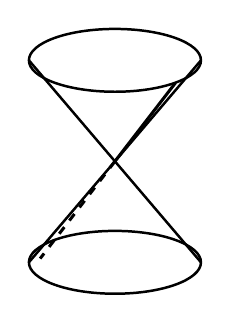
\begin{tikzpicture}[scale=0.95,line width=0.9pt]
  \draw (0,1.35) ellipse (1.15 and 0.42);
  \draw (0,-1.35) ellipse (1.15 and 0.42);
  \draw (-1.15,1.35) -- (0,0) -- (-1.15,-1.35);
  \draw (1.15,1.35) -- (0,0) -- (1.15,-1.35);
  \draw[line width=1.1pt] (0.81,1.05) -- (0,0);
  \draw[line width=1.1pt,dashed] (0,0) -- (-1.00,-1.30);
\end{tikzpicture}
\caption{$V(x,z)\subset\Spec k[x,y,z]/(xy-z^2)$ 是一张\trCone{}上的直线。（依原书手绘图重绘。）}\label{fig:cone-line-xyz}
\end{figure}

\textbf{13.1.4.}\ \emph{解答。}\quad 设 $\mathfrak{m}=(x,y,z)$ 是对应于原点的\trMaximalIdeal。于是 $\Spec A$ 在原点处的\trZariski{}\trTangentSpace{}具有\trDimension{} $3$，而 $\Spec A/(x,z)$ 在原点处的\trZariski{}\trTangentSpace{}具有\trDimension{} $1$。但由\mbox{练习~13.1.B}，$\Spec A/(f)$ 在原点处的\trZariski{}\trTangentSpace{}必定具有至少为 $2$ 的\trDimension。（附赠的收获是：我们顺便证明了 $A$ 不是\trUFD，依据是引理~12.1.7。\footnote{原书此处作（by Lemma 12.1.7.))），末尾衍一右括号，径删。——译者注}）

\textbf{13.1.5.}\ \hard\ \emph{\trhRemark{}。}\quad 解这道题还有另一条路，它不依赖\trZariski{}\trTangentSpace{}的定义：利用这个环是\trGrading{}的这一事实（其中 $x$、$y$、$z$ 的次数都是 $1$），且\trIdeal{} $(x,z)$ 是\trHomogeneous{}理想。（你也许会乐于亲自把这件事想一遍。）使用\trTangentSpace{}的优越性在于：它也适用于没有\trGrading{}的更一般的情形。例如，(a) $(x,z)$ 不是 $k[x,y,z]/(xy-z^2-z^3)$ 的\trPrincipalIdeal。作为另一个例子，(b) $(x,z)$ 不是\trLocalRing{} $(k[x,y,z]/(xy-z^2))_{(x,y,z)}$（「这张\trCone{}的\trGerm」）的\trPrincipalIdeal。然而我们提醒一句：分次情形仍然非常有用。把一个\trFiltered{}环换成其「\trAssociatedGraded」（associated graded）环的构造，可以把更一般的环变成\trGradedRing（并且可以用来把例子 (a) 化为分次情形）。\trCompletion{}的构造则可以把\trLocalRing{}变成\trGrading{}局部环（并且可以用来把例子 (b) 在本质上也化为分次情形）。\trFiltered{}环将在 \S13.9 中登场；\trAssociatedGraded{}构造将在我们讨论\trBlowup{}时（\S22.3）隐含地出现；而\trCompletion{}的诸多面向将在第 28 章中得到描述。

\textbf{13.1.D.（练习）}\quad 证明：$(x,z)\subset k[w,x,y,z]/(wz-xy)$ 是一个\trCodimension{}为 $1$ 却非\trPrincipalIdeal{}的\trIdeal，用的是解答~13.1.4 的方法。（这一情形的\trProjectivization{}——一张\trSmooth{}\trQuadricSurface{}上的一条直线——见\cref{fig:ruled-line-quadric}。）这个例子就是\mbox{练习~5.4.D}之后随即许诺的那一个。\mbox{练习~15.5.N}给出了一个改进：这个\trClosedSubset{} $x=z=0$ 甚至不是由单独一条方程\trSetTheoretic{}地切出的。

\begin{figure}[htbp]
\centering
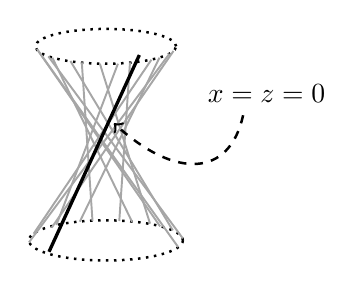
\begin{tikzpicture}[scale=0.85,line width=0.7pt]
  \draw[dotted,line width=0.9pt] (0,1.45) ellipse (1.05 and 0.26);
  \draw[dotted,line width=0.9pt] (0,-1.45) ellipse (1.15 and 0.30);
  \draw[gray!70] (-1.03,1.41) -- (1.08,-1.55);
  \draw[gray!70] (-0.86,1.30) -- (1.15,-1.42);
  \draw[gray!70] (-0.53,1.23) -- (1.00,-1.30);
  \draw[gray!70] (-0.09,1.19) -- (0.66,-1.20);
  \draw[gray!70] (0.36,1.21) -- (0.20,-1.16);
  \draw[gray!70] (0.80,1.28) -- (-0.39,-1.17);
  \draw[gray!70] (1.01,1.38) -- (-0.81,-1.26);
  \draw[gray!70] (-1.01,1.38) -- (0.81,-1.24);
  \draw[gray!70] (-0.80,1.28) -- (0.39,-1.17);
  \draw[gray!70] (-0.36,1.21) -- (-0.20,-1.16);
  \draw[gray!70] (0.18,1.19) -- (-0.74,-1.22);
  \draw[gray!70] (0.68,1.25) -- (-1.08,-1.35);
  \draw[gray!70] (0.95,1.34) -- (-1.15,-1.48);
  \draw[line width=1.2pt] (-0.85,-1.62) -- (0.50,1.32);
  \node at (2.40,0.75) {$x=z=0$};
  \draw[dashed,line width=0.9pt,->] (2.05,0.42) .. controls (1.85,-0.50) and (1.05,-0.55) .. (0.12,0.30);
\end{tikzpicture}
\caption{光滑\trQuadricSurface{} $V(wz-xy)\subset\mathbb{P}^3$ 上的直线 $V(x,z)$。（依原书手绘图重绘。）}\label{fig:ruled-line-quadric}
\end{figure}

\textbf{13.1.E.（练习）}\quad 设 $A=k[w,x,y,z]/(wz-xy)$。证明：$\Spec A$ 不是\trFactorial{}的。（\mbox{练习~5.4.L}表明 $A$ 不是\trUFD，但这还不够——为什么 $A$ 在素理想 $(w,x,y,z)$ 处的\trLocalization{}不是\trFactorial{}的？一种可能是「直接」做这件事，试着模仿\mbox{练习~5.4.L}的解法，但这很难。不如改用一条中间结果：在\trUFD{}中，任何\trCodimension{} $1$ 的\trPrimeIdeal{}都是\trPrincipalIdeal（引理~12.1.7），并结合\mbox{练习~13.1.D}来考虑。）由于当 $\operatorname{char}k\neq2$ 时 $A$ 是\trIntegrallyClosed{}的（\mbox{练习~5.4.I(c)}），这就给出了一个\trNormal{}却不\trFactorial{}的\trScheme{}的例子，正如\mbox{练习~5.4.F}所许诺的。稍作推广的版本将在\mbox{练习~22.4.N}中给出。

\textbf{13.1.F.（不甚重要的练习：「高阶数据」）}\quad （这个练习很有趣，但不会被用到。）
\begin{enumerate}[label=(\alph*)]
\item 在\mbox{练习~3.7.B}中，你计算过切出 $\mathbb{A}^3_k$ 的（并起来的）三条\trCoordinate{}轴的那些方程。（把这个\trScheme{}记作 $X$。）你的\trIdeal{}应当已经具有三个\trGenerator。证明：这个\trIdeal{}不能由更少的元素生成。（提示：模 $\mathfrak{m}=(x,y,z)$ 工作不会给出任何有用的信息，故请模 $\mathfrak{m}$ 的一个更高的幂工作。）
\item 证明：$\mathbb{A}^3_k$ 中的诸\trCoordinate{}轴到 $\mathbb{A}^3_k$ 中的嵌入并非\trRegularEmbedding。（这是 \S9.5 末尾所许诺的。）
\end{enumerate}

\textbf{13.1.6.}\ \emph{\trMorphism{}与\trTangentSpace。}\quad 设 $\pi\colon X\to Y$，且 $\pi(\mathrm{p})=\mathrm{q}$。假如我们身处可微流形的\trCategory，我们便会期待有一个切映射，从 $\mathrm{p}$ 的\trTangentSpace{}到 $\mathrm{q}$ 处的\trTangentSpace。事实也确实如此；我们有\trStalk{}的一个映射 $\OO_{Y,\mathrm{q}}\to\OO_{X,\mathrm{p}}$，它把前者的\trMaximalIdeal{} $\mathfrak{n}$ 送到后者的\trMaximalIdeal{} $\mathfrak{m}$（当我们简略地讨论\trLocallyRingedSpace{}时曾验证过这是一个「局部态射」；见 \S7.3.1）。于是 $\mathfrak{n}^2$ 被映到 $\mathfrak{m}^2$，由此我们见到 $\mathfrak{n}/\mathfrak{n}^2$ 被映到 $\mathfrak{m}/\mathfrak{m}^2$。若 $(\OO_{X,\mathrm{p}},\mathfrak{m})$ 与 $(\OO_{Y,\mathrm{q}},\mathfrak{n})$ 具有相同的\trResidueField{} $\kappa$，从而 $\mathfrak{n}/\mathfrak{n}^2\to\mathfrak{m}/\mathfrak{m}^2$ 是 $\kappa$-\trVectorSpace{}之间的一个线性映射，那么我们便有一个自然映射 $(\mathfrak{m}/\mathfrak{m}^2)^{\vee}\to(\mathfrak{n}/\mathfrak{n}^2)^{\vee}$。这就是我们所寻求的、从 $\mathrm{p}$ 的\trTangentSpace{}到 $\mathrm{q}$ 处的\trTangentSpace{}的映射。（旁注：注意\emph{余切}映射\emph{总是}存在，不要求 $\mathrm{p}$ 与 $\mathrm{q}$ 具有相同的\trResidueField——这正是一个信号，表明在\trAlgebraicGeometry{}中，\trCotangentSpace{}比\trTangentSpace{}更为自然。）

\textbf{13.1.G.（练习）}\quad 设 $X$ 是一个 $k$-\trScheme。描述从 $\Mor_k(\Spec k[\epsilon]/(\epsilon^2),X)$ 到如下数据的一个\trNatural{}\trBijection：一个具有\trResidueField{} $k$ 的点 $\mathrm{p}$（必是一个\trClosedPoint），以及 $\mathrm{p}$ 处的一个\trTangentVector。（这在例如形变理论（deformation theory）中很重要。我们不会用到它，所以你可以把它当作一件奇物。）

\textbf{13.1.H.（练习：好玩的算术操练）}\quad 求 $\mathbb{Z}[2i]\cong\mathbb{Z}[x]/(x^2+4)$ 中点 $[(2,2i)]$ 处\trZariski{}\trTangentSpace{}的\trDimension。再求 $\mathbb{Z}[\sqrt{-2}]\cong\mathbb{Z}[x]/(x^2+2)$ 中点 $[(2,x)]$ 处\trZariski{}\trTangentSpace{}的\trDimension。（若你更喜欢这些例子的几何版本，把 $\mathbb{Z}$ 换成 $\mathbb{C}$、把 $2$ 换成 $y$：考虑 $\mathbb{C}[x,y]/(x^2+y^2)$ 与 $\mathbb{C}[x,y]/(x^2+y)$。）

\textbf{13.1.7.\ 有限型情形下的一个重要诠释：\trJacobianMatrix{}\trCorank。}

\textbf{13.1.I.（重要练习：\trJacobianMatrix{}算出有理点处的\trZariski{}\trCotangentSpace）}\quad 设 $X$ 是一个\trFiniteType{} $k$-\trScheme。那么\trLocally{}地它形如 $\Spec k[x_1,\dots,x_n]/(f_1,\dots,f_r)$。证明：在一个 $k$-\trValuedPoint（即具有\trResidueField{} $k$ 的一个\trClosedPoint）处的\trZariski{}\trCotangentSpace，由「雅可比映射」（Jacobian map）$k^r\to k^n$ 的\trCokernel{}给出，而这个映射由 \textbf{\trJacobianMatrix}（Jacobian matrix）
\begin{equation*}\tag{13.1.7.1}\label{eq:jacobian-corank-matrix}
J=
\begin{pmatrix}
\dfrac{\partial f_1}{\partial x_1}(\mathrm{p}) & \cdots & \dfrac{\partial f_r}{\partial x_1}(\mathrm{p})\\
\vdots & \ddots & \vdots\\
\dfrac{\partial f_1}{\partial x_n}(\mathrm{p}) & \cdots & \dfrac{\partial f_r}{\partial x_n}(\mathrm{p})
\end{pmatrix}.
\end{equation*}
给出。（这把我们那道「$\mathbb{A}^3$ 中由几个方程切出一条\trCurve」的例子精确化了——在那里我们挑出了线性项；见例~13.1.2。）你可能会警觉：$\frac{\partial f}{\partial x_1}$ 究竟是什么\emph{意思}？你需要 $\delta$ 与 $\epsilon$ 吗？不需要！只需形式地定义导数即可，例如
\[
\frac{\partial}{\partial x_1}\bigl(x_1^2+x_1x_2+x_2^2\bigr)=2x_1+x_2.
\]
提示：先在 $\mathrm{p}$ 为原点时做这件事，并考虑线性项，正如例~13.1.2 与\mbox{练习~13.1.B}那样。至于一般情形，「把 $\mathrm{p}$ 平移到原点去」。

\textbf{13.1.8.}\ \emph{\trhRemark{}。}\quad 这条结果可以推广到\trResidueField{}在 $k$ 上\trSeparable{}的那些\trClosedPoint（特别地，若 $\operatorname{char}k=0$ 或 $k$ 有限，则可推广到\emph{全部}\trClosedPoint）；见注记~21.2.34。我们等到第 21 章才来证明这件事，并不意味着它必定如此复杂；一个更初等的证明是可能的。

\textbf{13.1.9.}\ \emph{\trhWarning{}。}\quad 在数学中更常见（但并不普遍）的做法，是把\trJacobianMatrix{}定义为 \eqref{eq:jacobian-corank-matrix} 的转置。

\textbf{13.1.J.（练习：\trJacobianMatrix{}的\trCorank{}不依赖于表述）}\quad 设 $A$ 是一个\trFinitelyGenerated{} $k$-\trAlgebra，由 $x_1,\dots,x_n$ 生成，其关系理想（ideal of relations）$I$ 由 $f_1,\dots,f_r$ 生成。设 $\mathrm{p}$ 是 $\Spec A$ 的一点。
\begin{enumerate}[label=(\alph*)]
\item 设 $g\in I$。证明：把 $g$ 的各偏导数组成的一列添到\trJacobianMatrix{} \eqref{eq:jacobian-corank-matrix} 上，不改变其在 $\mathrm{p}$ 处的\textbf{\trCorank}（corank）（即\trCokernel{}的\trDimension）。进而证明：\trJacobianMatrix{}在 $\mathrm{p}$ 处的\trCorank{}不依赖于 $I$ 的诸\trGenerator{}的选取。
\item 设 $q(x_1,\dots,x_n)$ 是 $k[x_1,\dots,x_n]$ 中的一个多项式。令 $h$ 为多项式 $y-q(x_1,\dots,x_n)\in k[x_1,\dots,x_n,y]$。证明：$(f_1,\dots,f_r,h)$ 关于变量 $(x_1,\dots,x_n,y)$ 的\trJacobianMatrix，在 $\mathrm{p}$ 处与 $(f_1,\dots,f_r)$ 关于 $(x_1,\dots,x_n)$ 的\trJacobianMatrix{}具有相同的\trCorank。进而证明：\trJacobianMatrix{}在 $\mathrm{p}$ 处的\trCorank{}不依赖于 $A$ 的诸\trGenerator{}的选取。
\end{enumerate}
于是，每个\trFiniteType{} $k$-\trScheme{} $X$ 都自带一个内蕴的「\textbf{\trJacobianMatrix{}\trCorank{}函数}」（Jacobian corank function），它从（$X$ 的\trUnderlyingSet{}）映到 $\mathbb{Z}^{\ge0}$，在 $X$ 的 $k$-\trValuedPoint{} $\mathrm{p}$ 处取值为 $\dim_\kappa\mathrm{T}_{X,\mathrm{p}}$。我们暂时把这个函数记作 $\mathrm{JC}\colon X\to\mathbb{Z}^{\ge0}$，尽管日后将会发现，它其实是\trDifferential{}的\trCoherentSheaf{} $\Omega_{X/\kappa}$ 的\trRank（\mbox{练习~21.2.E}）。

\textbf{13.1.K.（容易的练习）}\quad 证明：$\mathrm{JC}$ 是一个\trUpperSemicontinuous{}的函数。

\textbf{13.1.L.（练习）}\quad 证明：$\mathrm{JC}$ 在 $k$ 的\trFieldExtension{}之下保持。更精确地说，若 $X$ 是一个\trFiniteType{} $k$-\trScheme，$\ell/k$ 是一个\trFieldExtension，并且在\trBaseChange{}映射 $X\times_k\ell\to X$（$\mathrm{p}\mapsto\mathrm{q}$）之下，证明 $\mathrm{JC}(\mathrm{p})=\mathrm{JC}(\mathrm{q})$。

\textbf{13.1.M.（练习）}\quad 证明：对任意 $\mathrm{p}\in X$，$\mathrm{JC}(\mathrm{p})\ge\dim_X\mathrm{p}$。（此时 $X$ 必然在 $k$ 上\trFiniteType，但 $\mathrm{p}$ 不必是 $X$ 的\trClosedPoint。）$X$ 在 $\mathrm{p}$ 处的\trDimension，即 $\dim_X\mathrm{p}$，定义于\mbox{练习~12.2.K}。提示：先料理 $k=\overline{k}$ 的情形，在这里以诸\trClosedPoint{}为杠杆。然后再对一般的 $k$ 证明这条结果，办法是证明不等式两侧都在\trFieldExtension{}之下保持（\mbox{练习~13.1.L}与\mbox{练习~12.2.M}）。

\textbf{13.1.N.（练习：计算\trProjective{} $k$-\trScheme{}的\trJacobianMatrix{}\trCorank{}函数）}\quad 设 $X\subset\mathbb{P}^n_k$ 由\trHomogeneous{}多项式 $f_i\in k[x_0,\dots,x_n]$（$1\le i\le r$）切出。证明：$X$ 的\trJacobianMatrix{}\trCorank{}函数比「射影雅可比矩阵」（projective Jacobian matrix）的\trCorank{}恰小 $1$：
\begin{equation*}\tag{13.1.9.1}\label{eq:projective-jacobian-corank}
\mathrm{JC}(\mathrm{p})=\operatorname{corank}
\begin{pmatrix}
\dfrac{\partial f_1}{\partial x_0}(\mathrm{p}) & \cdots & \dfrac{\partial f_r}{\partial x_0}(\mathrm{p})\\
\vdots & \ddots & \vdots\\
\dfrac{\partial f_1}{\partial x_n}(\mathrm{p}) & \cdots & \dfrac{\partial f_r}{\partial x_n}(\mathrm{p})
\end{pmatrix}-1.
\end{equation*}
你必须设法让右端有意义，因为射影\trJacobianMatrix{}的元素并不是函数；这个\trCorank{}到底是什么意思呢？


\section{正则性与域上光滑}

\trRegularity{}定义中的关键想法，已包含在定理~12.3.12 之中（\trZariski{}\trTangentSpace{}的维数至少是\trLocalRing{}的维数）。

\textbf{13.2.1.}\ \emph{\trhDefinition{}。}\quad 若定理~12.3.12 中取等号，则称 $A$ 是一个\textbf{\trRegular\trLocalRing}（regular local ring）。特别地，\emph{\trRegular\trLocalRing{}按定义是\trNoetherian{}的}。（若一个\trNoetherian{}环 $A$ 在它的所有\trPrimeIdeal{}处都正则——也就是说，若对 $A$ 的所有\trPrimeIdeal{} $\mathfrak{p}$，$A_{\mathfrak{p}}$ 都是\trRegular\trLocalRing——则称 $A$ 是一个\textbf{\trRegular{}环}（regular ring）。这个术语我们基本不去使用。事实~13.8.2 令人安心地蕴涵：\trRegular\trLocalRing{}的确是\trRegular{}环。）一个\trLocally\trNoetherian{}概形 $X$ 称为在一点 $p$ 处是\textbf{正则}的（regular），若\trLocalRing{} $\OO_{X,p}$ 是正则的。（「\trNonsingular{}的」（nonsingular）一词也常被使用，特别是当 $X$ 是域上的\trFiniteType{}概形时；但为了口径一致，我们全篇使用「正则」。）否则称它在这一点处是\textbf{\trSingular{}的}（singular），并称这个点是一个\textbf{\trSingularPoint}（singularity）。（「非正则的」（nonregular）一词也在使用，但同样为了口径一致，我们将使用「\trSingular{}的」——尽管这个选择，与我们宁取「正则」而不取「\trNonsingular」的选择是\emph{不相一致}的。这种不相一致的一个可能的动机是：「正则局部环」与「\trSingularPoint」都是标准术语，所以总有个时刻我们不得不做出选择。）一个概形是\textbf{正则}的（regular）（或\textbf{\trNonsingular{}的}（nonsingular）），若它在所有点处都正则；否则它是\textbf{\trSingular{}的}（singular）（也就是说，它在\emph{至少一个}点处\trSingular——若它有一个\trSingularPoint）。

\textbf{13.2.A.（练习）}\quad 证明：维数为 $0$ 的\trNoetherian\trLocalRing{}正则，当且仅当它是一个域。

希望你将渐渐信服：这就是概形的「\trSmoothness」的正确观念。值得注意的是，\trKrull{}出于纯代数的理由引入了\trRegular\trLocalRing{}的观念，那比\trZariski{}于 1947 年认识到它是几何中的一个基本观念，还要早上一些时候。

\textbf{13.2.B.（练习）}\quad 设 $(A,\mathfrak{m})$ 是维数为 $n>0$ 的\trRegular\trLocalRing，而 $f\in A$。证明：$A/(f)$ 是维数为 $n-1$ 的\trRegular\trLocalRing，当且仅当 $f\in\mathfrak{m}\setminus\mathfrak{m}^2$。（提示：切空间版的\trKrull{}\trPrincipalIdealTheorem，\mbox{练习~13.1.B}。）

\textbf{13.2.C.（练习：\trRegularity{}的切片判别法）}\quad 设 $X$ 是一个\trNoetherian{}概形（例如一个\trVariety），$D$ 是 $X$ 上的一张\trEffectiveCartierDivisor（定义~9.5.1），而 $p\in D$。证明：若 $p$ 是 $D$ 的正则点，则 $p$ 是 $X$ 的正则点。（提示：切空间版的\trKrull{}\trPrincipalIdealTheorem，\mbox{练习~13.1.B}。）

\textbf{13.2.D.（容易的练习：操练概念）}\quad 设 $(A,\mathfrak{m})$ 是维数为 $d$ 的\trRegular\trLocalRing，而 $f_1,\dots,f_d\in\mathfrak{m}$，它们在\trVectorSpace{} $\mathfrak{m}/\mathfrak{m}^2$ 中的像构成一组基。证明：它们是 $(A,\mathfrak{m})$ 的一个\trSystemOfParameters（定义~12.3.11）。（它们是「特别好」的参数。）

\textbf{13.2.2.\ \trRegularity{}的\trJacobianCriterion。}

\trFiniteType{}的 $k$-\trScheme{}局部地都形如 $\Spec k[x_1,\dots,x_n]/(f_1,\dots,f_r)$。当 $k=\overline{k}$ 时，\trRegularity{}的\trJacobianCriterion（\mbox{练习~13.2.E}）给出一个可以动手操作的方法，利用方程 $f_1,\dots,f_r$ 来检验\trClosedPoint{}处的\trSingular{}性。

\textbf{13.2.E.（重要练习：\trRegularity{}的\trJacobianCriterion——有了\mbox{练习~13.1.I}便容易）}\quad 设 $X=\Spec k[x_1,\dots,x_n]/(f_1,\dots,f_r)$ 具有\trPureDimension{} $d$。证明：$k$-\trValuedPoint{} $p\in X$ 是正则的，当且仅当雅可比\trCorank{}函数在 $p$ 处取值为 $d$。

\textbf{13.2.F.（容易的练习）}\quad 设 $k=\overline{k}$。证明：$\mathbb{A}^n_k$ 中超曲面 $f(x_1,\dots,x_n)=0$ 的\trSingular\trClosedPoint{}由方程组
\[
f=\frac{\partial f}{\partial x_1}=\cdots=\frac{\partial f}{\partial x_n}=0
\]
给出。（转述：$f=0$ 的\trSingular{}点，就是 $f$ 的梯度消失之处。这一点也不令人震惊。）

\textbf{13.2.3.\ 域上的\trSmoothness。}

\trJacobianCriterion{}似乎有两个严重的缺陷。对 $\overline{k}$ 上的\trFiniteType{}概形，这条判别法给出了\trRegularity{}的一个必要条件，但其是否充分并不显然——我们还需要在非\trClosedPoint{}处也检验\trRegularity。我们可以通过费力证明事实~13.8.2 来证得充分性，该事实蕴涵：非\trClosedPoint{}也必是正则的。第二个缺陷是：这条判别法要求 $k$ 是\trAlgClosedField。这些问题让人以为：使用导数与雅可比矩阵的老式想法，配不上花哨的现代\trRegularity{}观念。但这样想就错了——毛病出在\trRegularity{}这个概念身上。有一个更好的观念：域上的\trSmoothness。更妙的是，这个观念还能推广到概形的\trSmooth\trMorphism{}观念（将在 \S13.6 中讨论，并将在第~24.8 章中再次讨论），它在一切可能的方面都表现良好（包括 \S8.1 的意义上）。这是又一个迹象，表明我们原以为属于对象的一些性质（「绝对观念」），其实应当被理解为态射的性质（「相对观念」）。我们已经懂得足够多，足以（不完美地、然而正确地）定义一个概形何时是\textbf{$k$-光滑}的，或\textbf{在 $k$ 上光滑}的了。

\textbf{13.2.4.}\ \emph{\trhDefinition{}。}\quad 一个 $k$-\trScheme{}称为 \textbf{维数 $d$ 的 $k$-光滑}（$k$-smooth of dimension $d$）概形，或 \textbf{在 $k$ 上维数为 $d$ 的光滑}（smooth of dimension $d$ over $k$）概形，若它具有\trPureDimension{} $d$，并且存在一个由\trAffine\trOpenSubset{} $\Spec k[x_1,\dots,x_n]/(f_1,\dots,f_r)$ 组成的\trCover，使\trJacobianMatrix{}在\emph{所有}点（而不仅在\emph{\trClosed{}点}）处的\trCorank{}为 $d$。（特别地，光滑概形不言而喻地是\trLocally\trFiniteType{}的。）一个 $k$-\trScheme{}称为\textbf{在 $k$ 上光滑}的（smooth over $k$），若它在某个维数下光滑。上下文清楚时，$k$ 常被省略。由 \S13.1.7 中发展的雅可比\trCorank{}函数理论，对任何\trPureDimension{}为 $d$ 的\trVariety，这一点可以在\emph{任何一个}\trAffine\trOpenCover{}上加以检验。

\textbf{13.2.G.（练习：最初的例子）}
\begin{enumerate}[label=(\alph*)]
\item 证明：对任何 $n$ 与任何域 $k$，$\mathbb{A}^n_k$ 都是光滑的。对哪些特征，$\mathbb{P}^2_k$ 中的曲线 $y^2z=x^3-xz^2$ 是光滑的（对照\mbox{练习~13.3.C}）？
\item 设 $f\in k[x_1,\dots,x_n]$ 是一个多项式，使得方程组
\[
f=\frac{\partial f}{\partial x_1}=\cdots=\frac{\partial f}{\partial x_n}=0
\]
在 $\overline{k}$ 中无解。证明：$\mathbb{A}^n_k$ 中的超曲面 $f=0$ 是光滑的。（把这道题与\mbox{练习~13.2.F}相比较，后者多出 $k=\overline{k}$ 这条假设。）
\end{enumerate}

\textbf{13.2.H.（练习：簇的光滑性「与基域的扩张无关」）}\quad 设 $X$ 是一个\trLocally\trFiniteType{}的 $k$-\trScheme，而 $k\subset\ell$ 是一个\trFieldExtension。证明：$X$ 在 $k$ 上光滑，当且仅当 $X\times_{\Spec k}\Spec\ell$ 在 $\ell$ 上光滑。

下一道练习表明：我们只需检验\trClosedPoint{}，从而与经典几何搭上了关系。

\textbf{13.2.I.（练习）}\quad 证明：若 $X=\Spec k[x_1,\dots,x_n]/(f_1,\dots,f_r)$ 的\trJacobianMatrix{}在所有\emph{\trClosed{}点}处的\trCorank{}为 $d$，则它在\emph{所有}点处的\trCorank{}为 $d$。（提示：\trJacobianMatrix{}\trCorank{}为 $d$ 的那个\trLocus，可以用某些显式矩阵的行列式的消失与非消失来描述。）

\textbf{13.2.5.}\ \emph{为\trRegularity{}辩护。}\quad 我们方才替\trSmoothness{}慷慨陈词，但也应当说清楚：\trRegularity{}仍然非常有用。例如，它是唯一在\trMixedCharacteristic（mixed characteristic）下说得通的概念。特别地，$\mathbb{Z}$ 在它的各个点处都正则（它是一个\trRegular{}环），而更一般地，\trDVR{}是\trRegular{}环的极其有用的例子。

\textbf{13.2.6.\ \trRegularity{}对\trSmoothness。}

\textbf{13.2.J.（练习）}\quad 设 $X$ 是\trAlgClosedField{} $k=\overline{k}$ 上\trPureDimension{}为 $d$ 的一个\trLocally\trFiniteType{}概形。证明：$X$ 在它的诸\trClosedPoint{}处正则，当且仅当它是光滑的。（我们很快就会知道：对\trLocally\trFiniteType{}的 $\overline{k}$-概形，闭点处的正则性与处处正则是一回事，见定理~13.8.3。）证明「正则蕴涵光滑」的提示：用\trJacobianCriterion{}证明\trJacobianMatrix{}的\trCorank{}在 $X$ 的诸\trClosedPoint{}处为 $d$，然后用\mbox{练习~13.2.I}。

更一般地，若 $k$ 是完全域（例如 $\operatorname{char}k=0$ 或 $k$ 是\trFinite{}域），则\trSmoothness{}与\trClosedPoint{}处的\trRegularity{}是一回事（见\mbox{练习~13.2.R}）。再更一般地，我们日后将证明下述事实。现在就把它摆出来，是因为远在最终证明它之前，它就能让一大批陈述变得干净利落。（不会有循环论证。）

\textbf{13.2.7.\ 光滑性--正则性比较定理。}\ ——
\begin{enumerate}[label=(\alph*)]
\item \emph{若 $k$ 是完全域，则每个正则的\trFiniteType{} $k$-\trScheme{}都在 $k$ 上光滑。}
\item \emph{每个光滑的 $k$-\trScheme{}都是正则的（对完全性不作任何假设）。}
\end{enumerate}

(a) 将在\mbox{练习~13.2.R}中证明。(b) 将在 \S24.8.9 中证明。定理~13.2.7(b) 要到那么遥远的将来才获证明，并不意味着我们真的得等那么久。我们是有意把证明推迟到手上有了能替我们做掉大部分工作的工具之时。如果你希望立刻得到一点洞见，这里是 (b) 的论证梗概；读完本章之后，你甚至可以试着把它实现出来。我们很快将证明（\mbox{练习~13.3.P}）：对一切域 $k$，$\mathbb{A}^n_k$ 都是正则的。一旦知道了\trEtale{}\trMorphism{}的定义，我们就会认识到：每个光滑\trVariety{}局部地都容有一个到 $\mathbb{A}^n_k$ 的\trEtale{}\trMorphism（观察~13.6.4）。那时你便能证明：若 $\pi\colon X\to Y$ 是\trLocally\trNoetherian{}概形之间的\trEtale{}\trMorphism，而 $p\in X$，则只要 $\pi(p)$ 正则，$p$ 就正则。这将在\mbox{练习~24.8.E}中获得证明，不过你在读完平展性的定义之后就去证明它，也毫不失当。

\textbf{13.2.8.}\ \emph{\trhCaveat{}：\trRegularity{}不蕴涵\trSmoothness。}\quad 若 $k$ 不是完全域，则\trRegularity{}\emph{不}蕴涵\trSmoothness，下面的例子即为明证。令 $k=\mathbb{F}_p(u)$，并考虑超曲面 $X=\Spec k[x]/(x^p-u)$。此时 $k[x]/(x^p-u)$ 是一个域，故而是正则的。但若 $f(x)=x^p-u$，则 $f(u^{1/p})=\frac{df}{dx}(u^{1/p})=0$，于是\trJacobianCriterion{}失效——$X$ \emph{在 $k$ 上}并不光滑。（千万别忘记：\trSmoothness{}需要一个域的选取——它是一个「相对」观念；日后我们将在 \S13.6 中定义任意概形上的\trSmoothness。）

\textbf{13.2.9.}\quad 倘若嫌上一个例子太「小」而不足以启人深思（因为所论概形在\emph{另一个}域上\emph{确}实光滑，即在 $k[x]/(x^p-u)$ 上光滑），这里再给出一个。同前取 $k=\mathbb{F}_p(u)$，但设 $p>2$，并考虑曲线 $\Spec k[x,y]/(y^2-x^p+u)$。那么\trClosedPoint{} $(y,x^p-u)$ 是正则的，却不光滑。

因此，你不要把「正则」与「光滑」当作同义词混用。

\textbf{13.2.10.\ \trRegular\trLocalRing{}都是\trIntegralDomain。}

凭几何直觉你或许会预期：概形在一个「光滑」的点处是「\trLocally\trIrreducible」的。用代数语言来说：

\textbf{13.2.11.\ \trhTheorem{}。}\ ——\ \emph{设 $(A,\mathfrak{m},k)$ 是维数为 $n$ 的\trRegular\trLocalRing。那么 $A$ 是一个\trIntegralDomain。}

在证明它之前（\S13.2.14），我们先给出几条推论。

\textbf{13.2.K.（练习）}\quad 设 $p$ 是一个\trLocally\trNoetherian{}概形 $X$ 的一个正则点。证明：$X$ 只有一个\trIrreducibleComponent{}经过 $p$。

\textbf{13.2.L.（容易的练习）}\quad 证明：非空的\trRegular\trNoetherian{}概形是\trIrreducible{}的，当且仅当它是\trConnected{}的。

\textbf{13.2.M.（重要练习：\trRegular{}概形之中的\trRegular{}概形是\trRegularEmbedding）}
\begin{enumerate}[label=(\alph*)]
\item 设 $(A,\mathfrak{m},k)$ 是维数为 $n$ 的\trRegular\trLocalRing，而 $I\subset A$ 是一个理想，它切出一个维数为 $d$ 的\trRegular\trLocalRing。令 $r=n-d$。证明：$\Spec A/I$ 是 $\Spec A$ 中的一个\trRegularEmbedding。提示：证明存在 $I$ 的元素 $f_1,\dots,f_r$，构成 $k$-\trVectorSpace{} $I/(I\cap\mathfrak{m}^2)$ 的一组基。证明：$A$ 分别对 $(f_1,\dots,f_r)$ 与对 $I$ 取商，得到的都是维数为 $d$ 的\trRegular\trLocalRing。由\mbox{练习~12.1.D}，同维数的\trIntegralDomain{}之间的满同态必是同构。
\item 设 $\pi\colon X\to Y$ 是正则概形之间的一个\trClosedEmbedding。证明：$\pi$ 是一个\trRegularEmbedding。
\end{enumerate}

\mbox{练习~13.2.M}有下面这个惊人的几何推论。

\textbf{13.2.N.（练习：推广\mbox{练习~12.3.F}）}
\begin{enumerate}[label=(\alph*)]
\item 设 $W$ 是\trAlgClosedField{} $k$ 上\trPureDimension{}为 $d$ 的一个光滑\trVariety，而 $X$ 与 $Y$ 是 $W$ 的\trCodimension{}分别为 $m$ 与 $n$ 的\trPureDimensional{}子簇（可以有\trSingularPoint）。证明：$X\cap Y$ 的每个分量在 $W$ 中的\trCodimension{}至多为 $m+n$，做法如下。证明对角 $W\cong\Delta\subset W\times_k W$ 是一个\trCodimension{}为 $d$ 的\trRegularEmbedding。然后照着\mbox{练习~12.3.F}的提示把其余步骤做完。（为什么对 $W$ 的假设是光滑而非正则？）
\item 从 (a) 中去掉 $k$ \trAlgClosed{}这一要求。
\end{enumerate}

\textbf{13.2.12.}\ \emph{\trhRemark{}。}\quad 下面的例子表明，\mbox{练习~13.2.N}中的光滑性假设不能（完全）去掉。令 $W=\Spec k[w,x,y,z]/(wz-xy)$ 为光滑\trQuadricSurface{}上的锥，它是一个\trIntegral{}的三维簇。令 $X$ 为曲面 $w=x=0$，$Y$ 为曲面 $y=z=0$；二者都含于 $W$。那么 $X\cap Y$ 恰为原点，于是我们有两个\trCodimension{} $1$ 的子簇相交于一个\trCodimension{} $3$ 的子簇。（$X$ 与 $Y$ 恰是同一\trRuling{}中两条直线的\trAffine{}锥，这绝非巧合；见\mbox{练习~9.3.L}。这个例子还将在\mbox{练习~22.4.N}中再度出现。）

\textbf{13.2.13.\ \trhProposition{}。}\ ——\ \emph{光滑的 $k$-\trScheme{}都是\trReduced{}的。}

这个论证蜿蜒得出奇！

\emph{证明。}\ 设 $X$ 是一个光滑的 $k$-\trScheme，并照常令 $X_{\overline{k}}:=X\times_{\Spec k}\Spec\overline{k}$。那么 $X_{\overline{k}}$ 是光滑的（\mbox{练习~13.2.H}），故 $X_{\overline{k}}$ 在其诸\trClosedPoint{}处正则（\mbox{练习~13.2.J}），故 $X_{\overline{k}}$ 在\trClosedPoint{}处的诸\trLocalRing{}都是\trIntegralDomain（定理~13.2.11），从而既约，于是 $X_{\overline{k}}$ 在其诸\trClosedPoint{}处既约、进而是既约的（\mbox{练习~5.2.E}或~6.6.N），故 $X$ 是既约的（你看出其中的缘由吗？）。\hfill$\square$

\textbf{13.2.O.（练习）}\quad 设 $p$ 是一个维数为 $n$ 的光滑 $k$-\trScheme{} $X$ 的一个\trClosedPoint。证明：$\OO_{X,p}$ 是一个\trIntegralDomain（其维数必为 $n$）。

\textbf{13.2.14.}\ \emph{定理~13.2.11 之证明（沿 [Liu, Prop.~2.11]）。}\quad 我们对 $n$ 作归纳。$n=0$ 的情形是清楚的（维数 $0$ 的\trRegular\trLocalRing{}是域，\mbox{练习~13.2.A}）。故设 $n>0$，且结论对更小的维数成立。

设 $\mathfrak{p}$ 是素理想，且 $\dim A/\mathfrak{p}=n$。我们要证 $\mathfrak{p}=(0)$。此时 $A/\mathfrak{p}$ 是一个维数为 $n$ 的\trNoetherian\trLocalRing，它的\trZariski{}\trCotangentSpace{}是 $A$ 者的一个商空间，由 $\mathfrak{p}$ 的「方程」切出（\mbox{练习~13.1.B}）。但 $\dim\mathfrak{m}/\mathfrak{m}^2=n$，故 $\mathfrak{p}\subset\mathfrak{m}^2$。于是 $A/\mathfrak{p}$ 是一个维数为 $n$ 的\trRegular\trLocalRing。

任取 $f\in\mathfrak{m}\setminus\mathfrak{m}^2$（于是 $f\notin\mathfrak{p}$）。由\mbox{练习~12.3.I}（同时应用于 $A/(f)$ 与 $A/(\mathfrak{p},f)$），$\dim A/(f)\ge n-1$，且 $\dim A/(\mathfrak{p},f)\ge n-1$，但这两个环的\trZariski{}\trTangentSpace{}的维数都是 $n-1$，故二者都是维数为 $n-1$ 的\trRegular\trLocalRing，再由归纳假设，二者都是\trIntegralDomain。一个\trIntegralDomain{}能够作为另一个同维数\trIntegralDomain{}的商，唯一的情形便是这个商是同构（\mbox{练习~12.1.D}）。于是 $(\mathfrak{p},f)=(f)$，从而 $\mathfrak{p}\subset(f)$，从而 $\mathfrak{p}\subset f\mathfrak{p}$，从而 $\mathfrak{p}=f\mathfrak{p}$。再由\trNakayama{}引理~8.2.9，$\mathfrak{p}=(0)$，正如所愿。\hfill$\square$

\textbf{13.2.15.}\ \extrahard\ \textbf{经基变换到 $\overline{k}$，在\trClosedPoint{}处检验 $k$-\trScheme{}的\trRegularity。}

（我们将在 21.2.Y 中以另一条思路重访这些想法，所以除非你格外好奇，否则不必读本小节。）\trJacobianCriterion{}是检验\trFiniteType{} $k$-\trScheme{}在 $k$-\trValuedPoint{}处\trRegularity{}的一条极好判别法。下面的结果把它的适用面推广到更一般的\trClosedPoint。

设 $X$ 是一个\trPureDimension{}为 $n$ 的\trFiniteType{} $k$-\trScheme，而 $p\in X$ 是一个\trResidueField{}为 $k'$ 的\trClosedPoint。由\trNullstellensatz~3.2.6，$k'/k$ 是域的一个\trFiniteFieldExtension。设它是可分的。定义 $\pi\colon X_{\overline{k}}:=X\times_k\overline{k}\to X$ 为由 $\Spec\overline{k}\to\Spec k$ 经基变换而来。

\textbf{13.2.P.（练习）}
\begin{enumerate}[label=(\alph*)]
\item 设 $f(x)\in k[x]$ 是一个\trSeparable{}多项式（即 $f$ 在 $\overline{k}$ 中有互不相同的根），且不可约，于是 $k'':=k[x]/(f(x))$ 是 $k$ 的一个\trFieldExtension。证明：作为环，$k''\otimes_k\overline{k}$ 就是 $\overline{k}\times\cdots\times\overline{k}$，其中因子的个数为 $\deg f=\deg k''/k$。
\item 证明：$\pi^{-1}(p)$ 由 $\deg(k'/k)$ 个\emph{既约}点组成。
\end{enumerate}

\textbf{13.2.Q.（练习）}\quad 设 $p$ 是 $X$ 的一个\trClosedPoint，其\trResidueField{} $k'$ 是 $k$ 的 $d$ 次\trSeparable{}扩张。证明：$X_{\overline{k}}$ 在 $p$ 的全部原像 $p_1,\dots,p_d$ 处都正则，当且仅当 $X$ 在 $p$ 处正则，做法如下。
\begin{enumerate}[label=(\alph*)]
\item 化归到 $X=\Spec A$ 的情形。
\item 设 $\mathfrak{m}\subset A$ 是对应于 $p$ 的\trMaximalIdeal。将正合列
\[
\begin{tikzcd}
0 \ar[r] & \mathfrak{m} \ar[r] & A \ar[r] & k' \ar[r] & 0
\end{tikzcd}
\]
与 $\overline{k}$ 作张量（域扩张保持向量空间序列的正合性），我们便得到正合列
\[
\begin{tikzcd}
0 \ar[r] & \mathfrak{m}\otimes_k\overline{k} \ar[r] & A\otimes_k\overline{k} \ar[r] & k'\otimes_k\overline{k} \ar[r] & 0.
\end{tikzcd}
\]
证明：$\mathfrak{m}\otimes_k\overline{k}\subset A\otimes_k\overline{k}$ 是对应于 $p$ 在 $\Spec A\otimes_k\overline{k}$ 中的\trPullback{}的那个理想。验证 $(\mathfrak{m}\otimes_k\overline{k})^2=\mathfrak{m}^2\otimes_k\overline{k}$。
\item 将 $k$-\trVectorSpace{}的短正合列
\[
\begin{tikzcd}
0 \ar[r] & \mathfrak{m}^2 \ar[r] & \mathfrak{m} \ar[r] & \mathfrak{m}/\mathfrak{m}^2 \ar[r] & 0
\end{tikzcd}
\]
与 $\overline{k}$ 作张量，证明
\[
\sum_{i=1}^{d}\dim_{\overline{k}}T_{X_{\overline{k}},p_i}=d\dim_{k'}T_{X,p}.
\]
\item 利用\mbox{练习~12.1.H(a)}以及不等式 $\dim_{\overline{k}}T_{X_{\overline{k}},p_i}\ge\dim X_{\overline{k}}$ 与 $\dim_{k'}T_{X,p}\ge\dim X$（定理~12.3.12）来得出结论。
\end{enumerate}

\textbf{13.2.16.}\ \emph{\trhRemark{}。}\quad 事实上，只要有单个 $p_i$ 处的正则性，便足以推出 $p$ 处的正则性。你可以接着\mbox{练习~13.2.Q}证明这一点：先处理 $k'/k$ 是\trGalois{}扩张的情形，并得到 $\operatorname{Gal}(k'/k)$ 在 $\{p_1,\dots,p_d\}$ 上的某个传递群作用。另一条路线见\mbox{练习~21.2.Y}。

\textbf{13.2.R.（练习）}\quad 设 $k$ 是完全域，而 $X$ 是一个\trFiniteType{} $k$-\trScheme。证明：$X$ 是光滑的，当且仅当 $X$ 在所有\trClosedPoint{}处正则。特别地，定理~13.2.7(a) 成立。提示：令 $X_{\overline{k}}:=X\times_k\overline{k}$。解释为什么：$X$ 光滑当且仅当 $X_{\overline{k}}$ 光滑，当且仅当 $X_{\overline{k}}$ 在所有\trClosedPoint{}处正则，当且仅当 $X$ 在所有\trClosedPoint{}处正则。最后一步见\mbox{练习~13.2.Q}。


\section{例子}

现在，我们通过一系列例子与练习，来实地考察\trRegularity{}与\trSmoothness。

\textbf{13.3.1.}\ \emph{几何例子。}

\textbf{13.3.A.（容易的练习）}\quad 设 $k$ 是一个域。证明：$\mathbb{A}^1_k$ 与 $\mathbb{A}^2_k$ 都是正则的，办法是直接检验所有点处的\trRegularity。证明：$\mathbb{P}^1_k$ 与 $\mathbb{P}^2_k$ 是正则的。

推广到任意维数则更难，我们把它留给\mbox{练习~13.3.P}。相比之下，$\mathbb{A}^n_k$ 与 $\mathbb{P}^n_k$ 是光滑的这件事基本上是一望即知的。

\textbf{13.3.B.（练习：射影超曲面正则性的\trJacobianCriterion）}
\begin{enumerate}[label=(\alph*)]
\item 证明：$\mathbb{P}^n_k$ 中超曲面 $f=0$ 的非光滑点对应于\trLocus
\[
f=\frac{\partial f}{\partial x_0}=\cdots=\frac{\partial f}{\partial x_n}=0.
\]
若这张超曲面的次数不被 $\operatorname{char}k$ 整除（例如当 $\operatorname{char}k=0$ 时），证明：只需检验 $\partial f/\partial x_0=\cdots=\partial f/\partial x_n=0$。提示：证明 $(\deg f)f=\sum_i x_i\frac{\partial f}{\partial x_i}$。
\item 若更进一步 $k=\overline{k}$，证明：奇\trClosedPoint{}由同一条轨迹给出。（事实上，这条轨迹给出的是全部\trSingularPoint，而不仅是奇闭点；参 \S13.2.3。我们用不到它，因此不证。）
\end{enumerate}

\textbf{13.3.C.（练习）}\quad 设 $\operatorname{char}k\neq2$。证明：$\mathbb{P}^2_k$ 中的 $y^2z=x^3-xz^2$ 是一条\trIrreducible{}的光滑\trCurve。（\trEisenstein{}判别法（Eisenstein's Criterion）给出了证明\trIrreducibility{}的一条途径。警告：我们并未规定 $\operatorname{char}k\neq3$，所以在使用\trJacobianCriterion{}时要当心。）

\textbf{13.3.D.（练习）}\quad 设 $\operatorname{char}k\neq2$。证明：$\mathbb{P}^n$ 中的二次超曲面是光滑的，当且仅当它具有极大秩（定义见\mbox{练习~5.4.J}）。

\textbf{13.3.E.（练习）}\quad 设 $k=\overline{k}$ 具有特征 $0$。证明：存在次数为 $d$ 的正则（射影）平面曲线。提示：试试「\trFermat{}曲线」$x^d+y^d+z^d=0$。（欢迎自行减弱这些假设。\trBertini{}定理~13.4.2 将给出证明存在性的另一条途径。）

\textbf{13.3.F.（练习，见\cref{fig:plane-curve-singularities}）}\quad 设 $k=\overline{k}$ 且 $\operatorname{char}k=0$，以免分心。求下述各平面曲线的奇\trClosedPoint（它们将是非光滑点）。
\begin{enumerate}[label=(\alph*)]
\item $y^2=x^2+x^3$。这是一个\emph{\trNode}的例子，我们在\mbox{练习~7.5.H}中见过。
\item $y^2=x^3$。这称为\emph{\trCusp}（cusp），我们在\mbox{练习~10.7.F}中见过它。
\item $y^2=x^4$。这称为\emph{\trTacnode}（tacnode），我们在\mbox{练习~10.7.G}中见过它。
\end{enumerate}

\begin{figure}[htbp]
\centering
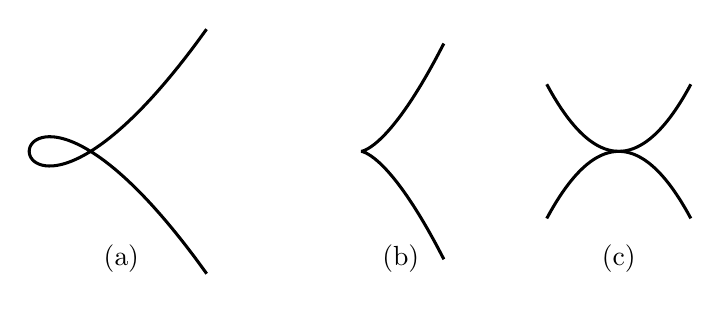
\begin{tikzpicture}[scale=0.78,line width=1.1pt]
  \begin{scope}
    \draw plot[smooth,variable=\t,domain=-1.7:1.7,samples=61]
      ({\t*\t-1},{0.62*(\t*\t*\t-\t)});
    \node at (0.5,-1.75) {(a)};
  \end{scope}
  \begin{scope}[xshift=4.4cm]
    \draw plot[smooth,variable=\t,domain=-1.3:1.3,samples=41]
      ({0.8*\t*\t},{0.8*\t*\t*\t});
    \node at (0.65,-1.75) {(b)};
  \end{scope}
  \begin{scope}[xshift=8.6cm]
    \draw plot[smooth,variable=\x,domain=-1.02:1.02,samples=41]
      ({1.15*\x},{1.05*\x*\x});
    \draw plot[smooth,variable=\x,domain=-1.02:1.02,samples=41]
      ({1.15*\x},{-1.05*\x*\x});
    \node at (0,-1.75) {(c)};
  \end{scope}
\end{tikzpicture}
\caption{平面曲线奇点。（依原书手绘图重绘。）}\label{fig:plane-curve-singularities}
\end{figure}

\textbf{13.3.2.}\ \emph{\trhRemark{}。}\quad 关于\trNode、\trCusp{}与\trTacnode，有几种可能的定义。当 $k=\overline{k}$ 时，一个合理的定义如下。设 $C$ 具\trPureDimension{} $1$，而 $p\in C$ 是一个\trClosedPoint。令 $(A,\mathfrak{m})$ 为\trLocalRing{} $\OO_{C,p}$，于是 $A/\mathfrak{m}=k$。我们称 $p$ 是 $C$ 的一个\textbf{\trNode}，若 $\dim_k\mathfrak{m}/\mathfrak{m}^2=2$，且
\[
\operatorname{Sym}^2(\mathfrak{m}/\mathfrak{m}^2)\longrightarrow\mathfrak{m}^2/\mathfrak{m}^3
\]
的\trKernel{}维数为 $1$，并且该\trKernel{}不由 $\mathfrak{m}/\mathfrak{m}^2$ 中某个元素的平方张成。这个定义我们用不到，所以你无须记住它。但你能弄明白它为什么合理吗？你能为\trCusp{}猜出一个合理的定义吗？关于\trNode、\trCusp{}及更多的另一些定义，将在 \S28.2 中给出。

\textbf{13.3.G.（练习）}\quad 证明：扭曲三次曲线 $\Proj k[w,x,y,z]/(wz-xy,\ wy-x^2,\ xz-y^2)$ 是光滑的。（你可以利用它与 $\mathbb{P}^1$ \trIsomorphic{}这一事实来做。但请用这些显式方程来做，以资练习。扭曲三次曲线定义于\mbox{练习~9.3.A}。）

\textbf{13.3.3.}\ \emph{\trTangentPlane{}与\trTangentLine。}\quad 设概形 $X\subset\mathbb{A}^n$ 由方程 $f_1,\dots,f_r$ 切出，而 $X$ 在 $k$-值点 $a=(a_1,\dots,a_n)$ 处是（纯）维数 $d$ 的光滑概形。那么\textbf{$X$ 在 $a$ 处的切 $d$-平面}（tangent $d$-plane to $X$ at $a$；有时记作 $T_aX$）便由 $r$ 条方程
\[
\biggl(\frac{\partial f_i}{\partial x_1}(a)\biggr)(x_1-a_1)+\cdots+\biggl(\frac{\partial f_i}{\partial x_n}(a)\biggr)(x_n-a_n)=0,
\]
给出，其中（如 \eqref{eq:jacobian-corank-matrix} 中那样）$\frac{\partial f_i}{\partial x_1}(a)$ 表示 $\frac{\partial f_i}{\partial x_1}$ 在 $a=(a_1,\dots,a_n)$ 处的取值。

\textbf{13.3.H.（练习）}\quad 为什么这与 $X$ 的定义方程 $f_1,\dots,f_r$ 的\emph{选取}无关？

\trRegularity{}的\trJacobianCriterion（\mbox{练习~13.2.E}）保证这 $r$ 条方程确实切出一个 $d$-平面。（当 $d=1$ 时，它称为\trTangentLine。）不难证明：这正是我们在多元微积分中所见到的那种\trTangentPlane{}观念\footnote{原书此处作（can be readily shown to be notion of tangent plane），当脱一「the」，径补。——译者注}。但请注意，在这里它是\emph{定义}，因此我们不必操心那些 $\delta$ 与 $\epsilon$。我们所需当心的只是：它要按我们期望的方式行事。

\textbf{13.3.I.（练习）}\quad 计算\mbox{练习~13.3.F(b)}的曲线在 $(1,1)$ 处的\trTangentLine。

\textbf{13.3.J.（练习）}\quad 计算\mbox{练习~13.3.G}的扭曲三次曲线在 $[1,1,1,1]$ 处的（射影）\trTangentLine。

\textbf{13.3.K.（练习）}\quad 设 $X\subset\mathbb{P}^n_k$（$k$ 照常是一个域）由\trHomogeneous{}方程 $f_1,\dots,f_r$ 切出，而 $p\in X$ 是一个（纯）维数为 $d$ 的光滑 $k$-值点。定义 $X$ 在 $p$ 处的（射影）切 $d$-平面。（定义~9.3.3 给出了 $\mathbb{P}^n_k$ 中 $d$-平面的定义，但你应当无须去查它。）

\textbf{13.3.4.}\ \emph{帮你把思路理清爽的旁注。}\quad 我们会希望切 $k$-平面的定义是自然的，其含义是：对 $\mathbb{A}^n_k$ 的任何\trAutomorphism{} $\sigma$（或者，在上一道练习的情形，$\mathbb{P}^n_k$ 的任何\trAutomorphism），都有 $\sigma(T_pX)=T_{\sigma(p)}\sigma(X)$。你可以动手直接验证这一点，但你也可以用更清爽的方式来说：以\trCoordinateFree{}的方式解读切出\trTangentSpace{}的那些方程。非正式地说，我们是在使用「$n$ 维空间」与「$n$ 维空间在 $p$ 处的\trTangentSpace」之间的\trCanonical{}等同，并且在利用这样一件事实：雅可比「\trLinearTransformation」切出 $T_p\mathbb{A}^n_k$ 中的 $T_pX$ 的方式，既不依赖于 $\mathbb{A}^n$ 上坐标的选取，也不依赖于我们对 $X$ 的定义方程。你对\mbox{练习~13.3.H}的解答，将有助于你开始以这种方式思考。

\textbf{13.3.L.（练习）}\quad 设 $X\subset\mathbb{P}^n_k$ 是由 $f=0$ 切出的一张次数为 $d$ 的超曲面，而 $L$ 是一条不含于 $X$ 的直线。\mbox{练习~9.3.D}（\trBezout{}定理的一个特例）表明：$X$ 与 $L$ 交于 $d$ 个点，按「重数」计入。设 $L$ 在一个 $k$-值点 $p\in L\cap X$ 处与 $X$ 相交的「重数至少为 $2$」，且 $p$ 是 $X$ 的正则点。证明：$L$ 含于 $X$ 在 $p$ 处的\trTangentPlane。（你的脑海里有一幅这样的图景吗？）

\textbf{13.3.5.}\ \emph{算术例子。}

\textbf{13.3.M.（容易的练习）}\quad 证明：$\Spec\mathbb{Z}$ 是一条正则\trCurve。

\textbf{13.3.N.（练习）}\quad （这道棘手的练习是为那些知道\textbf{\trGauss{}整数}（Gaussian integers）$\mathbb{Z}[i]$ 的诸素元的读者准备的。）证明 $\mathbb{Z}[i]$ 的维数为 $1$，办法有好几种。（例如：（i）它是一个\trPID；（ii）它是 $\mathbb{Z}$ 在域扩张 $\mathbb{Q}(i)/\mathbb{Q}$ 中的\trNormalization；（iii）用\trKrull{}\trPrincipalIdealTheorem~12.3.3 以及「$\dim\mathbb{Z}[x]=2$（\mbox{练习~12.1.I}）」这条事实。）证明：$\Spec\mathbb{Z}[i]$ 是一条正则\trCurve。（有好几条路可走。你可以用\mbox{练习~13.1.B}。作为一道可以先行演练的例子，考虑素理想 $(1+i)$，它在 $\Spec\mathbb{Z}[x]/(x^2+1)$ 中由方程 $1+x$ 切出。）日后（\S13.5.9）讨论了\trDVR{}之后，我们会有更简单的办法。

\textbf{13.3.O.（练习）}\quad 证明：$[(5,5i)]$ 是 $\Spec\mathbb{Z}[5i]$ 的唯一\trSingularPoint。（提示：$\mathbb{Z}[i]_5\cong\mathbb{Z}[5i]_5$。用上一道练习。）

\textbf{13.3.6.}\ \emph{回到几何：$\mathbb{A}^n_k$ 是正则的。}\quad 证明 $\mathbb{A}^n_k$（$k$ 是一个域）正则的关键一步，是下面这条。

\textbf{13.3.7.\ \trhProposition{}。}\ ——\ \emph{设 $(B,\mathfrak{n},k)$ 是维数为 $d$ 的\trRegular\trLocalRing。令 $\phi\colon B\to B[x]$。设 $\mathfrak{p}$ 是 $A:=B[x]$ 的一个\trPrimeIdeal，满足 $\mathfrak{n}B[x]\subset\mathfrak{p}$。那么 $A_{\mathfrak{p}}$ 是\trRegular\trLocalRing。}

\emph{证明。}\ 几何地说：我们有态射 $\pi\colon X=\Spec B[x]\to Y=\Spec B$，且 $\pi([\mathfrak{p}])=[\mathfrak{n}]$。纤维 $\pi^{-1}([\mathfrak{n}])$ 是 $\Spec(B[x]/\mathfrak{n}B[x])=\Spec k[x]$。于是，要么 (i) $[\mathfrak{p}]$ 是 $[\mathfrak{n}]$ 上方的纤维 $\mathbb{A}^1_k$，要么 (ii) $[\mathfrak{p}]$ 是纤维 $\mathbb{A}^1_k$ 的一个\trClosedPoint。（见\cref{fig:spec-bx-fiber}。）

\begin{figure}[htbp]
\centering
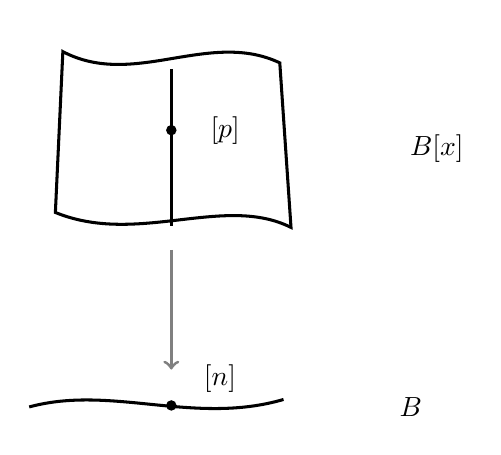
\begin{tikzpicture}[scale=0.95,line width=0.9pt]
  \draw[line width=1.1pt] (-1.55,2.75)
    .. controls (-0.6,2.25) and (0.4,3.05) .. (1.35,2.6)
    -- (1.5,0.4)
    .. controls (0.6,0.85) and (-0.55,0.15) .. (-1.65,0.6)
    -- cycle;
  \draw[line width=1.1pt] (-0.1,2.52) -- (-0.1,0.42);
  \fill (-0.1,1.7) circle (0.07);
  \node at (0.62,1.7) {$[\mathfrak{p}]$};
  \node at (3.45,1.45) {$\Spec B[x]$};
  \draw[gray,line width=1.1pt,->] (-0.1,0.1) -- (-0.1,-1.5);
  \draw[line width=1.1pt] (-2.0,-2.0)
    .. controls (-0.9,-1.7) and (0.2,-2.25) .. (1.4,-1.9);
  \fill (-0.1,-1.98) circle (0.07);
  \node at (0.55,-1.62) {$[\mathfrak{n}]$};
  \node at (3.1,-2.0) {$\Spec B$};
\end{tikzpicture}
\caption{命题~13.3.7 的证明背后的几何。（依原书手绘图重绘。）}\label{fig:spec-bx-fiber}
\end{figure}

在考虑这两种情形之前，我们先作两条注记。由于 $(B,\mathfrak{n})$ 是维数为 $d$ 的\trRegular\trLocalRing，$\mathfrak{n}$ 由 $B$ 的 $d$ 个元素生成，设为 $f_1,\dots,f_d$（\mbox{练习~13.2.D}），并且存在一条素理想链
\begin{equation*}\tag{13.3.7.1}\label{eq:regular-local-prime-chain}
0=\mathfrak{q}_0\subset\mathfrak{q}_1\subset\cdots\subset\mathfrak{q}_d=\mathfrak{n}.
\end{equation*}

\emph{情形 (i)：$[\mathfrak{p}]$ 是纤维 $\mathbb{A}^1_k$。}\ 在此情形，$\mathfrak{p}=\mathfrak{n}B[x]$。于是由\trKrull{}高度定理~12.3.10，$\mathfrak{p}=\mathfrak{n}B[x]$ 的\trCodimension{}至多为 $d$，因为 $\mathfrak{p}$ 由 $d$ 个元素 $f_1,\dots,f_d$ 生成。但 $\mathfrak{p}$ 的\trCodimension{}至少为 $d$：给定以 $\mathfrak{n}$ 收尾的链 \eqref{eq:regular-local-prime-chain}，我们在 $B[x]$ 中便有一条以 $\mathfrak{n}B[x]$ 收尾的相应素理想链。于是 $\mathfrak{p}$ 的\trCodimension{}恰为 $d$，而 $\mathfrak{p}A_{\mathfrak{p}}$ 由 $f_1,\dots,f_d$ 生成，这蕴含它是\trRegular\trLocalRing。

\emph{情形 (ii)：$[\mathfrak{p}]$ 是纤维 $\mathbb{A}^1_k$ 的一个\trClosedPoint。}\ $k[x]$ 的闭点 $\mathfrak{p}$ 对应于某个首一的不可约多项式 $g(x)\in k[x]$。把 $g$ 的系数任意提升到 $B$；我们马虎地把 $B[x]$ 中所得的多项式也记作 $g(x)$。于是 $\mathfrak{p}=(f_1,\dots,f_d,g)$，故由\trKrull{}高度定理~12.3.10，$\mathfrak{p}$ 的\trCodimension{}至多为 $d+1$。但 $\mathfrak{p}$ 的\trCodimension{}至少为 $d+1$：给定以 $\mathfrak{n}$ 收尾的链 \eqref{eq:regular-local-prime-chain}，我们在 $B[x]$ 中便有一条以 $\mathfrak{n}B[x]$ 收尾的相应链，再添上 $\mathfrak{p}$ 即可将其延长。于是 $\mathfrak{p}$ 的\trCodimension{}恰为 $d+1$，而 $\mathfrak{p}A_{\mathfrak{p}}$ 由 $f_1,\dots,f_d,g$ 生成，这蕴含它是\trRegular\trLocalRing。\hfill$\square$

\textbf{13.3.P.（练习）}\quad 用命题~13.3.7 证明：若 $X$ 是正则的（\trLocally\trNoetherian{}的）\trScheme，则 $X\times\mathbb{A}^1$ 亦是。特别地，证明 $\mathbb{A}^n_k$ 是正则的。（提示：想想纤维。）


\section{\trBertini{}定理}

现在我们来讨论\trBertini{}定理——一条基本的经典结果。

\textbf{13.4.1.}\ \emph{\trhDefinition{}：\trDualProjectiveSpace。}\quad $\mathbb{P}^n_k$（具有射影坐标 $x_0,\dots,x_n$）的\textbf{\trDual}（dual）（或\textbf{\trDualProjectiveSpace}（dual projective space）），非正式地说，就是 $\mathbb{P}^n_k$ 中\trHyperplane{}所成的空间。说得稍稍确切些：它是一个具有射影坐标 $a_0,\dots,a_n$ 的射影空间 $\mathbb{P}^n_k$（我们把它记作 $\mathbb{P}^{n\vee}_k$，徒劳地指望借此防止混淆），并附带如下数据：「\trIncidenceVariety」或「\trIncidenceCorrespondence」$I\subset\mathbb{P}^n\times\mathbb{P}^{n\vee}$，它由方程 $a_0x_0+\cdots+a_nx_n=0$ 切出。（这常称为\textbf{\trUniversalHyperplane}（universal hyperplane）。）注意：$\mathbb{P}^{n\vee}$ 的 $k$-值点确实对应于 $\mathbb{P}^n$ 中定义在 $k$ 上的那些\trHyperplane，而且这显然还是一种\trDuality{}关系（在定义中，$x$-变量与 $a$-变量之间存在着对称性）。这个定义足够具体，可供实践使用，并且能延拓到任意的\trBase（特别是 $\Spec\mathbb{Z}$）之上。（但如果你品味精致细腻，或许会想给出一个\trCoordinateFree{}的定义。）

\textbf{13.4.2.\ \trBertini{}定理。}\ ——\ \emph{设 $X$ 是 $\mathbb{P}^n_k$ 中（纯）维数为 $d$ 的一个\trSmooth\trClosed\trSubvariety。那么在\trDualProjectiveSpace $\mathbb{P}^{n\vee}_k$ 中存在一个非空（＝稠密）的\trOpenSubset{} $\mathcal{U}$，使得对每一点 $p=[H]\in\mathcal{U}$，概形 $H\cap X$ 在 $\kappa(p)$ 上光滑，且具有（纯）维数 $d-1$。}

（你或许应当先想想 $\kappa(p)=k$ 的情形，即 $H$ 是由一条系数取自 $k$ 的线性型所切出的\trHyperplane。）凡属这种风味的定理，常统称为「\trBertini{}定理」。一个例子是\trKleiman{}--\trBertini{}定理~21.6.10，它可\emph{不是}由\trKleiman{}与\trBertini{}二人联手证明的。

作为\trBertini{}定理~13.4.2 的一个应用：$\mathbb{P}^n_k$ 中一张一般的次数 $d>0$ 的超曲面与 $X$ 交出 $X$ 中\trCodimension{}为 $1$ 的一个光滑\trSubvariety：把 $X\hookrightarrow\mathbb{P}^n$ 换成复合
\[
\begin{tikzcd}
X \ar[r] & \mathbb{P}^n \ar[r, hook, "\nu_d"] & \mathbb{P}^N,
\end{tikzcd}
\]
其中 $\nu_d$ 是第 $d$ 次\trVeroneseEmbedding{}（9.3.8）。这里「一般」取其在\trAlgebraicGeometry{}中的惯常含义；见 \S10.3.7。（\mbox{练习~13.4.B}给出一个推广。）这样做的一个有用推论是：取 $X=\mathbb{P}^n$，我们立即看到 $\mathbb{P}^n$ 中存在光滑的次数 $d$ 超曲面（在任何无穷域 $k$ 上），而无须同具体的方程纠缠（\mbox{练习~13.3.E}即其特殊情形）。

\mbox{练习~21.6.I}给出了特征 $0$ 时\trBertini{}定理的一个有用的改进（见\mbox{练习~21.6.J}）。

\emph{证明。}\ 这条证明的中心想法相当朴素。我们将把那些「坏的」超平面描述出来，并证明它们构成 $\mathbb{P}^{n\vee}_k$ 的一个维数至多为 $n-1$ 的闭子集，从而其补集是一个稠密开子集。说得稍稍确切些：我们将定义一个射影簇 $Z\subset X\times\mathbb{P}^{n\vee}_k$，它可以非正式地描述为
\begin{equation*}\tag{13.4.2.1}\label{eq:bertini-bad-locus-z}
\begin{split}
Z=\bigl\{(p\in X,\ H\subset\mathbb{P}^n_k)&\ :\ p\in H,\\
&\text{并且 }p\text{ 是 }H\cap X\text{ 的\trSingularPoint，或者 }X\subset H\bigr\}.
\end{split}
\end{equation*}
我们将见到：投射 $\pi\colon Z\to X$ 在闭点处的纤维是维数为 $n-1-\dim X$ 的射影空间，从而 $\dim Z\le n-1$。于是 $Z$ 在 $\mathbb{P}^{n\vee}$ 中的像将是（定理~8.4.10）一个维数至多为 $n-1$ 的闭子集，故其补集既开又非空。现在我们就把这一策略付诸实施。

\textbf{13.4.3.}\quad 我们首先更精确地定义 $Z$，即通过 $\mathbb{P}^n\times\mathbb{P}^{n\vee}$ 上的方程来定义：$\mathbb{P}^n$ 上的坐标是 $x_0,\dots,x_n$，而 $\mathbb{P}^{n\vee}$ 上的对偶坐标是 $a_0,\dots,a_n$。设 $X$ 由 $f_1,\dots,f_r$ 切出。那么我们就取这些方程作为 $Z$ 的定义方程中的第一批。（至此我们定义了子概形 $X\times\mathbb{P}^{n\vee}$。）我们再添加方程 $a_0x_0+\cdots+a_nx_n=0$。（至此我们描述了 $\mathbb{P}^n\times\mathbb{P}^{n\vee}$ 中由点 $(p,H)$——其中 $p\in X$ 且 $p\in H$——所对应的子概形。）注意：射影\trJacobianMatrix{} \eqref{eq:projective-jacobian-corank}
\[
\begin{pmatrix}
\dfrac{\partial f_1}{\partial x_0}(p) & \cdots & \dfrac{\partial f_r}{\partial x_0}(p)\\
\vdots & \ddots & \vdots\\
\dfrac{\partial f_1}{\partial x_n}(p) & \cdots & \dfrac{\partial f_r}{\partial x_n}(p)
\end{pmatrix}
\]
由射影雅可比\trCorank{}判别法（\mbox{练习~13.1.N}）知，在 $X$ 的所有点处的\trCorank{}恰为 $d+1$。于是我们要求：在射影\trJacobianMatrix{}上添加新的一列
\[
\begin{pmatrix} a_0\\ \vdots\\ a_n \end{pmatrix}
\]
之后，所得矩阵的\trCorank{}不小于 $d+1$（因而 $=d+1$）。这恰是我们要捕捉的观念——你明白这是为什么吗？它由若干方程切出（某些\trMinor{}的行列式）。（注记~13.4.4 完整地走了一遍例子，或许有助于澄清这里的运作方式。）

我们接着证明 $\dim Z\le n-1$。对每个\trClosedPoint{} $p\in X$，令 $W_p$ 为包含 $p$、且满足「$H\cap X$ 在 $p$ 处\trSingular，或 $H$ 包含整个 $X$」的那些超平面所成的\trLocus；$W_p$ 的维数是多少？设 $\dim X=d$。那么 $W_p$ 的定义中对超平面的限制相应于 $d+1$ 个线性条件。（你明白为什么吗？）这意味着 $W_p$ 是一个\trCodimension{}为 $d+1$（也就是维数为 $n-d-1$）的射影空间。于是 $\pi\colon Z\to X$ 在每个\trClosedPoint{}上的纤维都具有纯维数 $n-d-1$。由\mbox{关键练习~12.4.A}，这蕴含 $\dim Z\le n-1$。（如果你愿意，可以用\mbox{练习~12.4.D}证明 $\dim Z=n-1$；并且日后等你知道了什么是射影丛（定义~17.2.4），还可以证明 $Z$ 是 $X$ 上的一个射影丛。但本证明用不到这些。）\hfill$\square$

\textbf{13.4.4.}\ \emph{\trhRemark{}。}\quad 这里有一个例子，或许有助于让你确信：段落~13.4.3 中的代数确实描述了我们想要的几何。考虑特征不为 $2$ 的域上的平面\trConic{} $x_0^2-x_1^2-x_2^2=0$；从坐标卡 $U_0$ 中的实图像着眼，你不妨把它想象成圆 $x^2+y^2=1$。考虑点 $[1,1,0]$，它对应于圆上的 $(1,0)$。我们期待仿射平面中的\trTangentLine{}是 $x=1$，它相应于 $x_0-x_1=0$。让我们看看代数给了我们什么。射影\trJacobianMatrix{}为
\[
\begin{pmatrix} 2x_0\\ -2x_1\\ -2x_2 \end{pmatrix}
=\begin{pmatrix} 2\\ -2\\ 0 \end{pmatrix},
\]
它果然如预期般具有秩 $1$。我们的配方要求矩阵
\[
\begin{pmatrix} 2 & a_0\\ -2 & a_1\\ 0 & a_2 \end{pmatrix}
\]
具有秩 $1$（即 $a_0=-a_1$ 且 $a_2=0$），并且还要求 $a_0x_0+a_1x_1+a_2x_2=0$，而这（请你自行核验）恰是我们想要的。

\textbf{13.4.A.（容易的练习）}
\begin{enumerate}[label=(\alph*)]
\item 在较弱的假设「$X$ 只有有限多个非光滑点」之下证明\trBertini{}定理。
\item 在较弱的假设「$X\to\mathbb{P}^n_k$ 是\trLocallyClosedEmbedding（但 $X$ 仍光滑）」之下证明\trBertini{}定理。
\end{enumerate}

\textbf{13.4.B.（练习：多超曲面的\trBertini{}定理）}\quad 设 $X$ 是 $\mathbb{P}^n_k$ 中（纯）维数为 $d\ge r$ 的一个光滑\trSubvariety。设 $e_1,\dots,e_r$ 是正整数，于是
\begin{equation*}\tag{13.4.4.1}\label{eq:multi-hypersurfaces-param}
\mathbb{P}^{\binom{e_1+n}{n}-1}\times\cdots\times\mathbb{P}^{\binom{e_r+n}{n}-1}
\end{equation*}
参数化了次数分别为 $e_1,\dots,e_r$ 的超曲面所成的 $r$ 元组 $(H_1,\dots,H_r)$。证明：存在 \eqref{eq:multi-hypersurfaces-param} 的一个稠密开子集 $\mathcal{U}$，使得对每一点 $p=[(H_1,\dots,H_r)]\in\mathcal{U}$，$H_1\cap\cdots\cap H_r\cap X$ 在 $\kappa(p)$ 上光滑，且具有（纯）维数 $d-r$。非正式地说：对次数分别为 $e_1,\dots,e_r$ 的超曲面 $H_1,\dots,H_r$ 作一般选取，则 $H_1\cap\cdots\cap H_r\cap X$ 光滑，且具有（纯）维数 $d-r$。（提示：不要去套用\trBertini{}定理~13.4.2，而是试着给出「同样的」证明。）这道练习的要点不在于要你记住这个具体结果，而在于：凡你需要的那类结果，你都有能力亲手证明。

\textbf{13.4.C.（练习）}\quad 设 $X$ 是 $\mathbb{P}^n$ 中维数为 $d$ 的一个射影簇，带有一个光滑的稠密开子集。（若基域完全，这件事会自动成立：见关于簇的一般光滑性（generic smoothness）的定理~21.6.1。）证明：$X$ 与 $d$ 张一般\trHyperplane{}的交由有限多个既约点组成。更精确地说：若 $\mathbb{P}^{n\vee}$ 是\trDualProjectiveSpace，则存在一个非空的\trZariski{}开子集 $\mathcal{U}\subset(\mathbb{P}^{n\vee})^d$，使得对 $\mathcal{U}$ 的每个\trClosedPoint{} $(H_1,\dots,H_d)$，概形论交 $H_1\cap\cdots\cap H_d\cap X$ 由有限多个既约点组成。（这样的点的个数——按正确方式计数——称为该簇的\trDegree；见\mbox{练习~18.6.M}。）

\textbf{13.4.5.}\ \emph{\trDualVariety。}\quad 我们关于\trBertini{}定理的讨论，给了我们一个顺便提及一个经典构造的借口。$Z$（见 \eqref{eq:bertini-bad-locus-z}）在 $\mathbb{P}^{n\vee}$ 中的像称为 $X$ 的\textbf{\trDualVariety}（dual variety）。由于 $\dim Z=n-1$，我们「期待」$X$ 的对偶是 $\mathbb{P}^{n\vee}$ 中的一张超曲面。这是一个并不显然的事实：这确实是一种\trDuality——$X$ 的对偶的对偶就是 $X$ 自身（见 [H2, Thm.~15.24]）。下面这道练习会让你对\trDualVariety{}有几分感觉。

\textbf{13.4.D.（练习）}\quad 证明：$\mathbb{P}^n$ 中一张\trHyperplane{}的对偶，就是对偶空间 $\mathbb{P}^{n\vee}$ 中那个相应的点。如此一来，$\mathbb{P}^n$ 与 $\mathbb{P}^{n\vee}$ 之间的对偶，便是射影簇之间对偶的一个特例。

\textbf{13.4.E.（练习）}\quad 设 $C\subset\mathbb{P}^2$ 是特征不为 $2$ 的\trAlgClosedField{}上的一条光滑\trConic。证明：$C$ 的\trDualVariety{}也是一条光滑\trConic。于是，举例来说，过平面上一个一般点（若 $k=\overline{k}$），有 $C$ 的两条切线。（对偶平面中一条直线上的诸点，对应于原平面中过某一点的那些直线。）

\textbf{13.4.F.}\ \hard\ \textbf{（练习：恰有一条光滑\trConic{}与五条一般直线相切，及其推广）}\quad 沿用上一题的记号，证明：含 $i$ 个一般选定的点、且与 $5-i$ 条一般选定的直线相切的光滑\trConic{} $C$ 的个数，当 $i=0$、$1$、$2$、$3$、$4$、$5$ 时，分别为 $1$、$2$、$4$、$4$、$2$、$1$。你不妨借助\trConic{}与对偶\trConic{}之间的对偶，来解读这个数列的对称性。这一事实恐怕早在旧石器时代就已为人所知了。


\section{离散\trValuationRing{}与代数哈托格斯引理}

（余）维数 $1$ 的情形是重要的，因为如果你懂得了被维数 $1$ 隔开的诸\trPrimeIdeal{}如何行事，那么你就可以用归纳法证明任意维数下的事实。这正是\trKrull{}\trPrincipalIdealTheorem~12.3.3 如此有用的原因之一。

一个维数为 $1$ 的\trRegular\trLocalRing{}可以被看作「一条\trSmooth{}\trCurve{}的\trGerm」（见\cref{fig:germ-of-curve}）。心里可以记着两个例子：$k[x]_{(x)}=\{f(x)/g(x)\ :\ x\nmid g(x)\}$ 与 $\mathbb{Z}_{(5)}=\{a/b\ :\ 5\nmid b\}$。第一个例子是「几何的」，第二个例子是「算术的」，但希望显然的是：二者有某种根本的共同点。

\begin{figure}[htbp]
\centering
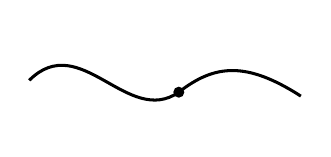
\begin{tikzpicture}[line width=1.1pt]
  \draw (-1.7,0.05) .. controls (-1.05,0.70) and (-0.45,-0.55) .. (0.20,-0.10) .. controls (0.65,0.25) and (1.05,0.30) .. (1.75,-0.15);
  \fill (0.20,-0.10) circle (0.07);
\end{tikzpicture}
\caption{一条\trCurve{}的\trGerm。（依原书手绘图重绘。）}\label{fig:germ-of-curve}
\end{figure}

本节的目的，是给出这些环的一长串彼此等价的定义。在开始之前，我们先把这七个定义迅速勾画一遍。一个\trNoetherian\trLocalRing{}可以「好」起来的方式有好几种。它可以是\trRegular{}的，可以是\trPID，可以是\trUFD，也可以是\trNormal{}的。在维数 $1$ 时，这些说法彼此相同。同样等价的是关于\trIdeal{}的几条好性质：$\mathfrak{m}$ 是\trPrincipalIdeal；或者\emph{所有}\trIdeal{}要么是\trMaximalIdeal{}的幂，要么是 $0$。最后，这个环可以带有一个离散\trValuation（discrete valuation）——一种对元素「大小」的度量，其表现格外良好。

\textbf{13.5.1.\ \trhTheorem{}。}\ ——\ \emph{设 $(A,\mathfrak{m})$ 是维数为 $1$ 的\trNoetherian\trLocalRing。则下列诸条彼此等价。}
\begin{enumerate}[label=(\alph*)]
\item \emph{$(A,\mathfrak{m})$ 是\trRegular{}的。}
\item \emph{$\mathfrak{m}$ 是\trPrincipalIdeal。}
\end{enumerate}

\emph{证明。}\ (a) 蕴涵 (b) 的理由如下。若 $A$ 正则，则 $\mathfrak{m}/\mathfrak{m}^2$ 是一维的。任取一个元素 $t\in\mathfrak{m}\setminus\mathfrak{m}^2$。那么 $t$ 生成 $\mathfrak{m}/\mathfrak{m}^2$，于是由\trNakayama{}引理~8.2.H，它生成 $\mathfrak{m}$（由\trNoetherian{}假设，$\mathfrak{m}$ 是有限生成的）。我们把这样的元素称为一个\textbf{\trUniformizer}（uniformizer）。

反过来，若 $\mathfrak{m}$ 在 $A$ 上由一个元素 $t$ 生成，则 $\mathfrak{m}/\mathfrak{m}^2$ 在 $A/\mathfrak{m}=k$ 上由一个元素 $t$ 生成。由定理~12.3.12，$\dim_k\mathfrak{m}/\mathfrak{m}^2\ge1$，于是 $\dim_k\mathfrak{m}/\mathfrak{m}^2=1$，所以 $(A,\mathfrak{m})$ 是正则的。\hfill$\square$

我们马上会用到一条有用的事实，它由几何动机驱动，并且是一条重要结果——\trArtin--\trRees（Artin--Rees）引理~13.9.3 的特例。我们将在 \S13.9 中证明它。

\textbf{13.5.2.\ \trhProposition{}。}\ ——\ \emph{若 $(A,\mathfrak{m})$ 是\trNoetherian\trLocalRing，则 $\bigcap_i\mathfrak{m}^i=0$。}

\textbf{13.5.3.}\quad 几何直观是：在一个点处「解析地为零」的函数（在各阶都消失）实际上在该点的一个开邻域内消失。（\mbox{练习~13.9.B}将把这件事说得更精确。）这个几何直观还提示了一个例子，表明\trNoetherian{}性是必要的：考虑 $\mathbb{R}$ 上原点处 $C^{\infty}$ 函数的芽环中的 $e^{-1/x^2}$。（特别地，这蕴涵：$\mathbb{R}$ 上 $C^{\infty}$ 函数的环在原点处的\trLocalization{}不是\trNoetherian{}的！）

人们忍不住想论证
\begin{equation*}\tag{13.5.3.1}\label{eq:m-powers-intersection}
\mathfrak{m}\bigl(\textstyle\bigcap_i\mathfrak{m}^i\bigr)=\textstyle\bigcap_i\mathfrak{m}^i,
\end{equation*}
然后用\trNakayama{}引理~8.2.9 论证 $\bigcap_i\mathfrak{m}^i=0$。遗憾的是，第一个等式是否为真并不显然：一般地，乘法与无穷递降交并不交换。（旁注：一般地，乘法与有限交也不交换，例如在 $k[x,y,z]/(xz-yz)$ 中，$(z)\bigl((x)\cap(y)\bigr)\neq(xz)\cap(yz)$。）我们将在\mbox{练习~13.9.A(b)} 中建立命题~13.5.2。（其实我们本可以现在就直接证明它，不太费事。）

\textbf{13.5.4.\ \trhTheorem{}。}\ ——\ \emph{设 $(A,\mathfrak{m})$ 是维数为 $1$ 的\trNoetherian\trLocalRing。则 (a) 与 (b) 等价于：}
\begin{enumerate}[label=(\alph*),start=3]
\item \emph{$A$ 是一个\trIntegralDomain，并且所有\trIdeal{}都具有形状 $\mathfrak{m}^n$（$n\ge0$）或 $(0)$。}
\end{enumerate}

\emph{证明。}\ 设 (a) 成立：设 $(A,\mathfrak{m},k)$ 是一个维数为 $1$ 的\trRegular\trLocalRing。我声称：对任何 $n$ 都有 $\mathfrak{m}^n\neq\mathfrak{m}^{n+1}$。否则，由\trNakayama{}引理，$\mathfrak{m}^n=0$，从而 $t^n=0$。但 $A$ 是\trIntegralDomain（由定理~13.2.11），于是 $t=0$，从而 $A=A/\mathfrak{m}$ 是一个域，而域的维数不是 $1$，矛盾。

我接着声称 $\mathfrak{m}^n/\mathfrak{m}^{n+1}$ 的维数为 $1$。理由：$\mathfrak{m}^n=(t^n)$。于是 $\mathfrak{m}^n$ 作为 $A$-模由一个元素生成，而 $\mathfrak{m}^n/(\mathfrak{m}\mathfrak{m}^n)$ 作为 $(A/\mathfrak{m}=k)$-模由一个元素生成（由上一段，它非零），所以它是一个一维\trVectorSpace。

于是我们有\trIdeal{}链 $A\supset\mathfrak{m}\supset\mathfrak{m}^2\supset\mathfrak{m}^3\supset\cdots$，满足 $\bigcap\mathfrak{m}^i=(0)$（命题~13.5.2）。我们想说：除这些之外，再没有别的\trIdeal{}的容身之处，因为每一对都被「维数 $1$」隔开，而且「末端没有余地」。证明：设 $I\subset A$ 是一个\trIdeal。若 $I\neq(0)$，则存在某个 $n$，使得 $I\subset\mathfrak{m}^n$ 但 $I\not\subset\mathfrak{m}^{n+1}$。取 $u\in I\setminus\mathfrak{m}^{n+1}$。那么 $(u)\subset I$。但 $u$ 生成 $\mathfrak{m}^n/\mathfrak{m}^{n+1}$，于是由\trNakayama{}引理它生成 $\mathfrak{m}^n$，所以我们得到 $\mathfrak{m}^n\subset I\subset\mathfrak{m}^n$，证毕：(c) 成立。

现在我们来证明 (c) 蕴涵 (a)。设 (a) 不成立：设我们有一个维数为 $1$ 的\trNoetherian{}局部\trIntegralDomain，它不正则，于是 $\mathfrak{m}/\mathfrak{m}^2$ 的维数至少为 $2$。任取 $u\in\mathfrak{m}-\mathfrak{m}^2$。那么 $(u,\mathfrak{m}^2)$ 是一个\trIdeal，但 $\mathfrak{m}^2\subsetneq(u,\mathfrak{m}^2)\subsetneq\mathfrak{m}$。\hfill$\square$

\textbf{13.5.A.（容易的练习）}\quad 设 $(A,\mathfrak{m})$ 是维数为 $1$ 的\trNoetherian\trLocalRing。证明：上面的 (a)--(c) 均等价于：
\begin{enumerate}[label=(\alph*),start=4]
\item \emph{$A$ 是一个\trPID。}
\end{enumerate}

\textbf{13.5.5.\ \trDVR。}\quad 我们接下来定义\trDVR{}的观念。设 $K$ 是一个域。$K$ 上的一个\textbf{离散\trValuation}（discrete valuation）是一个满同态 $v\colon K^{\times}\to\mathbb{Z}$（特别地，$v(xy)=v(x)+v(y)$），它满足
\[
v(x+y)\ge\min\bigl(v(x),v(y)\bigr)
\]
除非 $x+y=0$（此时左边无定义）。（这样的\trValuation{}称为\emph{\trNonArchimedean}的（non-Archimedean），尽管我们不会使用这个术语。）写下 $v(0)=\infty$ 往往是方便的。更一般地，一个\textbf{\trValuation}（valuation）是一个到全序\trAbelian{}群 $G$ 的满同态 $v\colon K^{\times}\to G$，尽管这对我们来说不那么重要。记号「val」将用来表示\trValuation。

这里有三个关键例子。
\begin{enumerate}[label=(\roman*)]
\item \emph{（$5$~进\trValuation）}$K=\mathbb{Q}$，$v(r)$ 是「出现在 $r$ 中的 $5$ 的幂」，例如 $v(35/2)=1$、$v(27/125)=-3$。
\item $K=k(x)$，$v(f)$ 是「出现在 $f$ 中的 $x$ 的幂」。
\item $K=k(x)$，$v(f)$ 是次数的相反数。这其实与 (ii) 是同一回事，只需把 $x$ 换成 $1/x$。
\end{enumerate}

于是 $\{0\}\cup\{x\in K^{\times}\ :\ v(x)\ge0\}$ 是一个环，我们把它记作 $\OO_v$。它称为 $v$ 的\textbf{\trValuationRing}（valuation ring）。（并非每个\trValuation{}都是离散的。考虑某个域 $k$ 上的\emph{\trPuiseux{}级数}（Puiseux series）环，$K=\bigcup_{n\ge1}k\bigl((x^{1/n})\bigr)$，\trValuation $v\colon K^{\times}\to\mathbb{Q}$ 由 $v(x^q)=q$ 给出。）

\textbf{13.5.B.（练习）}\quad 描述上面三个例子 (i)--(iii) 中的\trValuationRing。（你会注意到，它们是眼熟的维数为 $1$ 的\trNoetherian\trLocalRing。多么巧合！）

\textbf{13.5.C.（练习）}\quad 证明：$\{0\}\cup\{x\in K^{\times}\ :\ v(x)>0\}$ 是这个\trValuationRing{}的唯一\trMaximalIdeal。（提示：证明补集中的每个元素都可逆。）于是，\trValuationRing{}是一个局部环。

设 $A$ 是一个\trIntegralDomain。若存在其\trFractionField{} $K=K(A)$ 上的一个离散\trValuation $v$ 使得 $\OO_v=A$，则称 $A$ 是一个\textbf{\trDVR}（discrete valuation ring，简称 DVR）。类似地，若存在 $K$ 上的一个\trValuation $v$ 使得 $\OO_v=A$，则称 $A$ 是一个\textbf{\trValuationRing}。

现在，若 $A$ 是维数为 $1$ 的\trRegular\trLocalRing，而 $t$ 是一个\trUniformizer（作为\trIdeal{}生成 $\mathfrak{m}$ 的一个元素，或者等价地，作为 $k$-\trVectorSpace{}生成 $\mathfrak{m}/\mathfrak{m}^2$ 的一个元素），那么 $A$ 的任何非零元素 $r$ 都落在某个 $\mathfrak{m}^n\setminus\mathfrak{m}^{n+1}$ 中，于是 $r=t^nu$，其中 $u$ 可逆（因为 $t^n$ 生成 $\mathfrak{m}^n$——由\trNakayama{}引理——而 $r$ 也如此），所以 $K(A)=A_t=A[1/t]$。于是\emph{$K(A)^{\times}$ 的任何元素都可以唯一地写成 $ut^n$}，其中 $u$ 可逆，$n\in\mathbb{Z}$。这样我们就可以定义一个\trValuation $v$：$v(ut^n)=n$。

\textbf{13.5.D.（练习）}\quad 证明：$v$ 是一个离散\trValuation。

\textbf{13.5.E.（练习）}\quad 反过来，设 $(A,\mathfrak{m})$ 是一个\trDVR。证明：$(A,\mathfrak{m})$ 是维数为 $1$ 的\trRegular\trLocalRing。（提示：证明诸\trIdeal{}都形如 $(0)$ 或 $I_n=\{r\in A\ :\ v(r)\ge n\}$，而 $(0)$ 与 $I_1$ 是仅有的两个\trPrimeIdeal。于是我们便有\trNoetherian{}性，以及维数 $1$。证明：$I_1/I_2$ 由 $I_1-I_2$ 中任何一个元素的像生成。）

于是我们证明了：

\textbf{13.5.6.\ \trhTheorem{}。}\ ——\ \emph{\trIntegralDomain{} $A$ 是满足 (a)--(d) 的维数为 $1$ 的\trNoetherian\trLocalRing，当且仅当}
\begin{enumerate}[label=(\alph*),start=5]
\item \emph{$A$ 是一个\trDVR。}
\end{enumerate}

\textbf{13.5.F.（练习）}\quad 证明：一个\trDVR{}上只有一个离散\trValuation。

\textbf{13.5.7.}\ \emph{\trhDefinition{}。}\quad 于是，任何维数为 $1$ 的\trRegular\trLocalRing{}都自带其\trFractionField{}上的一个唯一\trValuation。若一个元素的\trValuation{}为 $n>0$，我们称该元素有一个 $n$ \textbf{阶\trZeros}（zero of order）。若\trValuation{}为 $-n<0$，我们称该元素有一个 $n$ \textbf{阶\trPole}（pole of order）。在处理完 (f) 与 (g) 之后，我们马上会回到这件事。

\textbf{13.5.8.\ \trhTheorem{}。}\ ——\ \emph{设 $(A,\mathfrak{m})$ 是维数为 $1$ 的\trNoetherian\trLocalRing。则 (a)--(e) 均等价于：}
\begin{enumerate}[label=(\alph*),start=6]
\item \emph{$A$ 是一个\trUFD，}
\item \emph{$A$ 是一个\trIntegralDomain，并且在（其\trFractionField{}中）整闭。}
\end{enumerate}

\emph{证明。}\ (a)--(e) 显然蕴涵 (f)，因为我们有下面这种「愚蠢的」唯一分解：$A$ 的每个非零元素都可以唯一地写成 $ut^n$，其中 $n\in\mathbb{Z}^{\ge0}$，$u$ 可逆。

(f) 蕴涵 (g)，因为\trUFD{}在其\trFractionField{}中是整闭的（\mbox{练习~5.4.F}）。

剩下要检验 (g) 蕴涵 (a)--(e)。我们将证明 (g) 蕴涵 (b)。

设 $(A,\mathfrak{m})$ 是维数为 $1$ 的\trNoetherian{}局部\trIntegralDomain，在其\trFractionField{} $K(A)$ 中整闭。任取非零的 $r\in\mathfrak{m}$。那么 $S=A/(r)$ 是一个维数为 $0$ 的\trNoetherian\trLocalRing——它唯一的素是 $\mathfrak{m}$ 的像，为避免混淆我们把它记作 $\mathfrak{n}$。于是 $\mathfrak{n}^N=0$，其中 $N$ 充分大（命题~12.1.9）。从而存在某个 $n$，使得 $\mathfrak{n}^n=0$ 而 $\mathfrak{n}^{n-1}\neq0$。

现在到了论证的关键之处。于是在 $A$ 中，$\mathfrak{m}^n\subset(r)$ 但 $\mathfrak{m}^{n-1}\not\subset(r)$。取 $s\in\mathfrak{m}^{n-1}-(r)$。考虑 $s/r\in K(A)$。由于 $s\notin(r)$，有 $s/r\notin A$，而 $A$ 是整闭的，所以 $s/r$ 不在 $A$ 上整。

现在（在 $K(A)$ 之内）$\frac{s}{r}\mathfrak{m}\not\subset\mathfrak{m}$（否则 $\frac{s}{r}\mathfrak{m}\subset\mathfrak{m}$ 将蕴涵 $\mathfrak{m}$ 是一个忠实 $A[\frac{s}{r}]$-模，与\mbox{练习~8.2.I}矛盾）。但 $s\mathfrak{m}\subset\mathfrak{m}^n\subset rA$，所以 $\frac{s}{r}\mathfrak{m}\subset A$。于是 $\frac{s}{r}\mathfrak{m}=A$，由此 $\mathfrak{m}=\frac{r}{s}A$，所以 $\mathfrak{m}$ 是\trPrincipalIdeal。\hfill$\square$

\textbf{13.5.9.}\ \emph{例：$\Spec\mathbb{Z}[i]$ 是正则的。}\quad 对于「$\Spec\mathbb{Z}[i]$ 为何正则」（\mbox{练习~13.3.N}），我们现在有了一个更简单的解释。首先，$\mathbb{Z}[i]$ 是\trUFD（\S5.4.5(o)），从而是\trNormal{}的（\S5.4.6）。它的维数为 $1$，于是由定理~13.5.8，它的闭点（即余维数 $1$ 的点）都正则。它的\trGenericPoint{}也正则，因为 $\mathbb{Z}[i]$ 是一个\trIntegralDomain。

\textbf{13.5.10.}\ \emph{例：「曲线几乎处处正则」。}\quad 由定理~13.5.8 与\mbox{练习~10.7.O}，每个一维\trVariety{}都除去有限多个\trClosedPoint{}外正则。

\textbf{13.5.11.}\ \emph{题外话：\trDedekindDomain。}\quad 一个\textbf{\trDedekindDomain}（Dedekind domain）是一个维数至多为 $1$ 的\trNoetherian\trIntegralDomain，它是\trNormal{}的（在其\trFractionField{}中整闭）。把一个\trDedekindDomain{}在除 $(0)$ 以外的任何一个素（即余维数 $1$ 的素）处取\trLocalization，得到的便是一个\trDVR。这是一个重要的概念，但我们不会多用它。数域的\trRingOfIntegers{}就是例子；见 \S10.7.1。特别地，若 $n$ 是一个模 $4$ 同余于 $3$ 的\trSquareFree{}整数，则 $\mathbb{Z}[\sqrt{n}]$ 是\trDedekindDomain（\mbox{练习~5.4.I(a)}）。如果你愿意，你可以证明\emph{\trDedekindDomain{}中\trIdeal{}的唯一分解}：非零理想都可以唯一地分解成\trPrimeIdeal。（提示：\trJordan--\trHolder{}的成套结果，\S6.5。）用与 \S13.5.9 中相同的论证，可知\trDedekindDomain{}都是正则的。

\textbf{13.5.12.\ \trNoetherian{}概形上函数的\trZeros{}与\trPole。}\quad 我们现在来推广下面这件事的说法：$\mathbb{A}^1_\mathbb{C}$ 上的 $(x-2)^2/(x-3)^4$ 在 $x=2$ 处有一个二阶\trZeros，在 $x=3$ 处有一个四阶极点。

\textbf{13.5.13.}\ \emph{\trhDefinition{}：余维数 $1$ 处正则（$\mathrm{R}_1$）。}\quad 我们称一个\trNoetherian{}环 $A$ 是\textbf{在余维数 $1$ 处正则}的（regular in codimension 1，简称 $\mathrm{R}_1$），若它在所有余维数 $1$ 的素处的\trLocalization{}都是\trRegular\trLocalRing。我们称一个\trLocally\trNoetherian{}概形 $X$ 是\textbf{在余维数 $1$ 处正则}的（regular in codimension 1，简称 $\mathrm{R}_1$），若它在它的余维数 $1$ 的点处正则。由定理~13.5.8，\trNoetherian{}正规概形都在余维数 $1$ 处正则。

\textbf{13.5.14.}\ \emph{\trhDefinition{}：在 $\mathrm{R}_1$ 点处的\trValuation。}\quad 设 $X$ 是一个\trLocally\trNoetherian{}概形\footnote{原书此处把该局部诺特概形记作（scheme $A$）（与同段环 $A$ 相撞），当系 $X$ 之误，径改。——译者注}。那么，对任何一个正则的余维数 $1$ 的点 $p$（即任何使 $\OO_{X,p}$ 成为维数为 $1$ 的\trRegular\trLocalRing{}的点 $p$），我们都有一个离散\trValuation $\mathit{val}_p$。若 $f$ 是 $\OO_{X,p}$ 的\trFractionField{}的任何一个非零元素（例如，若 $X$ 是整的，而 $f$ 是 $X$ 的\trFunctionField{}的一个非零元素），则当 $\mathit{val}_p(f)>0$ 时，我们称 $f$ \textbf{在 $p$ 处有} $\mathit{val}_p(f)$ \textbf{阶\trZeros}；而当 $\mathit{val}_p(f)<0$ 时，我们称 $f$ \textbf{在 $p$ 处有} $-\mathit{val}_p(f)$ \textbf{阶\trPole}。（我们尚不容许在一个并非正则的余维数 $1$ 点处讨论消失阶。定义倒是可以作出来，但它的表现可不如有离散\trValuation{}时那么好。\footnote{原书此处作（when have you have a discrete valuation），「have」当系衍词，径删。——译者注}）你能看出为什么 $75/34$ 在 $5$ 处有一个二阶\trZeros、在 $2$ 处有一个一阶极点吗？你能描述 $x^3(x+y)/(x^2+y)^3$ 在 $\mathbb{A}^2_k$ 上的\trZeros{}与极点吗？

\textbf{13.5.G.（练习：\trNoetherian{}概形上\trZeros{}与极点的有限性）}\quad 设 $X$ 是一个整的\trNoetherian{}概形，而 $f\in K(X)^{\times}$ 是其\trFunctionField{}的一个非零元素。证明：$f$ 只有有限多个\trZeros{}与极点。（提示：化归到 $X=\Spec A$。若 $f=f_1/f_2$，其中 $f_i\in A$，先对每个 $f_i$ 证明这条结果。）

\textbf{13.5.15.}\ \emph{\trhRemark{}。}\quad 一个（\trNoetherian{}）概形可以在余维数 $2$ 处\trSingular{}却依然\trNormal。例如，你已经证明过：在特征不为 $2$ 时，$\mathbb{A}^3$ 中的锥面 $x^2+y^2=z^2$ 是\trNormal{}的（\mbox{练习~5.4.I(b)}），但它在原点处\trSingular（\trZariski{}\trTangentSpace{}一眼望去就是三维的）。

但正规概形的奇性在某些方面并不算太糟：我们很快（\S13.5.18）就会为\trNoetherian{}正规概形讨论代数\trHartogs{}引理~13.5.19，它说的是：你可以把函数越过余维数 $2$ 的集合延拓出去。

\textbf{13.5.16.}\ \emph{\trhRemark{}。}\quad 我们知道，对\trNoetherian{}环有如下蕴含关系：
\[
\text{唯一分解整环}\;\Longrightarrow\;\text{整闭}\;\Longrightarrow\;\text{在余维数~1 处正则}
\]
于是，对\trLocally\trNoetherian{}概形，我们也有类似的蕴含关系：
\[
\text{唯一分解}\;\Longrightarrow\;\text{正规}\;\Longrightarrow\;\text{在余维数~1 处正则}
\]
这里有两个例子，向你表明这些包含关系都是严格的。

\textbf{13.5.H.（练习：\trPinchedPlane）}\quad 设 $A$ 是 $k[x,y]$ 的子环 $k[x^3,x^2,xy,y]$。（非正式地说：我们容许一切不含单项式 $x$ 的非零倍数的多项式。）证明：$\Spec k[x,y]\to\Spec A$ 是一个\trNormalization。证明：$A$ 不是整闭的。证明：$\Spec A$ 在余维数 $1$ 处正则。（最后一部分的提示：证明它是二维的，而当你把「原点」扔掉之后，得到的东西是正则的——办法是分别对 $x^2$ 与 $y$ 取逆，并考虑 $A_{x^2}$ 与 $A_y$。）

\textbf{13.5.17.}\ \emph{例（二次曲面再度登场）。}\quad 设 $k$ 是特征不为 $2$ 的\trAlgClosedField。那么 $k[w,x,y,z]/(wz-xy)$ 是整闭的，却不是\trUFD；见\mbox{练习~5.4.L}（以及\mbox{练习~13.1.E}）。

\textbf{13.5.18.\ \trNoetherian{}正规概形的代数\trHartogs{}引理。}\quad 多复变中的\trHartogs{}引理（非正式地）说：在一个余维数 $2$ 的集合之外定义的全纯函数，可以越过该集合延拓。我们现在来描述一个代数的类比，适用于\trNoetherian{}正规概形。（把它与黎曼第二延拓定理（Second Riemann Extension Theorem）作一番有益的比较也是可能的。）在 \S15.4 中把\trLineBundle{}与\trDivisor{}联系起来时，我们将反复地、不遗余力地使用这条结果。

\textbf{13.5.19.\ 代数\trHartogs{}引理。}\ ——\ \emph{设 $A$ 是一个整闭的\trNoetherian\trIntegralDomain。则}
\[
A=\bigcap\nolimits_{\mathfrak{p}\ \text{余维数 }1}A_{\mathfrak{p}}.
\]

这个等式在 $K(A)$ 之中成立；回忆：一个\trIntegralDomain{} $A$ 的任何\trLocalization{}都自然地是 $K(A)$ 的一个子集（\mbox{练习~1.2.C}）。警告：很少有人把这条引理称作代数\trHartogs{}引理。我这样称呼它，是因为它与复几何中的相应命题平行。

有人或许会这样说：若 $f\in K(A)$ 不落在 $A_{\mathfrak{p}}$ 中，其中 $\mathfrak{p}$ 的余维数为 $1$，则 $f$ 在 $[\mathfrak{p}]$ 处有一个极点；而若 $f\in K(A)$ 落在 $\mathfrak{p}A_{\mathfrak{p}}$ 中，其中 $\mathfrak{p}$ 的余维数为 $1$，则 $f$ 在 $[\mathfrak{p}]$ 处有一个\trZeros。

\textbf{13.5.20.}\quad 把代数\trHartogs{}引理在几何上解读为下述说法是值得的：\emph{\trNoetherian{}正规概形上没有极点的\trRationalFunction{}实际上是正则的（即它是 $A$ 的一个元素）。}非正式地说：「\trNoetherian{}正规概形具有\trHartogs{}性质。」

人们可以把代数\trHartogs{}引理更一般地陈述在 $\Spec A$ 是\trNoetherian{}正规概形的情形，意思是 $A$ 是若干个\trNoetherian{}正规\trIntegralDomain{}的乘积；读者不妨一试。

另一条推广（并且是某种更接近「正确」陈述的东西）是：若 $A$ 是域 $K$ 的一个子环，则 $A$ 在 $K$ 中的整闭包是 $K$ 的所有包含 $A$ 的\trValuationRing{}之交；说明与证明见 [AtM, Cor.~5.22]。

\textbf{13.5.21.}\ \hard\ \emph{代数\trHartogs{}引理~13.5.19 之证明。}\quad 证明中关键的妙招是下述构造。若 $A$ 是一个\trIntegralDomain，而 $r\in K(A)$，则 $r\in A$ 当且仅当对 $A$ 的所有\trPrimeIdeal{} $\mathfrak{p}$ 都有 $r\in A_{\mathfrak{p}}$，也就是说，$r$ 在 $\Spec A$ 的所有点处都正则。因此，问 $r\in K(A)$ 在哪些点处不正则是有意义的。我们的「分母理想」构造（来自命题~5.4.2\footnote{原书此处作（from the proof Proposition 5.4.2），当脱一「of」，径补。——译者注}的证明）表明这是一个闭子集：若 $I=\{a\in A\ :\ ar\in A\}$，则 $V(I)=\Supp A/I$ 的那些点 $[\mathfrak{p}]$ 恰好是 $r$ 不正则的点。我们从一个易于定义的模 $M^{a/b}$ 出发，可以对这个闭子集获得更精细的理解。

\textbf{13.5.22.}\quad 设 $r=a/b\notin A$，其中 $a,b\in A$。令 $\bar{a}$ 为 $a$ 在 $A/(b)$ 中的像。$r\notin A$ 这一事实意味着在 $A/(b)$ 中 $\bar{a}\neq0$。令 $M^{a/b}$ 为 $A/(b)$ 的由 $\bar{a}$ 生成的 $A$-子模。我们这样构造 $M^{a/b}$，使得 $M^{a/b}_q=0$ 当且仅当 $a/b\in A_q$\footnote{原书本节下标用斜体 $q$，而同段括注中又用 fraktur $\mathfrak{p}$（如 $A_{\mathfrak{p}}$），两种字形并存系原书自身不一致，兹照录。——译者注}。（翻译一下：$a$ 不是 $b$ 在 $A_{\mathfrak{p}}$ 中的倍数，当且仅当在 $A_{\mathfrak{p}}/(b)$ 中 $\bar{a}\neq0$。）

我们想证明代数\trHartogs{}引理，它说的是：若 $A$ 是整闭的，那么只需转而检验高度为 $1$ 的那些\trPrimeIdeal{}就够了。我们先给出这条事实的一个近似版本，它在没有「整闭」假设时也成立。

\textbf{13.5.23.\ \trhLemma{}。}\ ——\ \emph{设 $A$ 是一个\trNoetherian\trIntegralDomain，$r\in K(A)$。那么 $r\in A$ 当且仅当：对每个非零的 $g\in A$ 的每个\trPrimeIdeal{} $\mathfrak{p}\in\operatorname{Ass}(A/(g))$，都有 $r\in A_{\mathfrak{p}}$。}

\emph{证明。}\ 若 $r\in A$，则显然对一切 $\mathfrak{p}$ 都有 $r\in A_{\mathfrak{p}}$。故设 $r=a/b\notin A$。我们要找出一个这样的 $\mathfrak{p}$，使得 $r\notin A_{\mathfrak{p}}$，正如引理陈述中所描述的那样。我们取 $\mathfrak{p}$ 为 \S13.5.22 中构造的非零模 $M^{a/b}$ 的任一\trAssociatedPrimeIdeal。由于 $M^{a/b}$ 是 $A/(b)$ 的一个子模，$\mathfrak{p}$ 也是 $A/(b)$ 的\trAssociatedPrimeIdeal（\mbox{练习~6.6.G(a)}）。\hfill$\square$

\textbf{13.5.24.\ \trhProposition{}。}\ ——\ \emph{若 $A$ 是一个\trNoetherian{}整闭\trIntegralDomain，则}
\begin{enumerate}[label=(\roman*)]
\item \emph{$A$ 在余维数 $1$ 处正则（定义~13.5.13），}
\item \emph{对任何 $b\in A$，$A$-模 $A/(b)$ 没有\trEmbeddedPoint。}
\end{enumerate}

\emph{证明。}\ (i) 整闭性在\trLocalization{}下保持（\mbox{练习~5.4.A}），于是对每个余维数 $1$ 的素 $\mathfrak{p}$，$A_{\mathfrak{p}}$ 是整闭的。从而由定理~13.5.8，$A_{\mathfrak{p}}$ 正则。

(ii) 设 $\mathfrak{p}$ 是 $A/(b)$ 的一个\trAssociatedPrimeIdeal。我们想证明 $\mathfrak{p}$ 在 $A$ 中的余维数为 $1$。把 $A$ 换成其\trLocalization{} $A_{\mathfrak{p}}$，陈述的真值不变，所以只需证明下面这件事：「设 $(A,\mathfrak{m})$ 是一个\trNoetherian\trLocalRing，它是一个整闭\trIntegralDomain，且 $b\in\mathfrak{m}\setminus\{0\}$。设 $\mathfrak{m}\in\operatorname{Ass}(A/(b))$。那么 $\mathfrak{m}$ 是\trPrincipalIdeal（从而余维数至多为 $1$）。」

我们现在来证明这段话。取 $\bar{a}\in A/(b)$ 使得 $\operatorname{Ann}(\bar{a})=\mathfrak{m}$。那么 $\bar{a}\neq0$。把 $\bar{a}$ 提升为 $a\in A$。那么 $a/b\in K(A)\setminus A$，并且 $(a/b)\mathfrak{m}\subset A$。

我们用反证法证明 $(a/b)\mathfrak{m}\not\subset\mathfrak{m}$。假设不然。回忆\mbox{练习~8.2.I}：「设 $A$ 是 $K$ 的一个子环，$r\in K$，而 $N$ 是一个忠实 $A[r]$-模，它作为 $A$-模是有限生成的。那么 $r$ 在 $A$ 上整。」我们在这里以 $r=a/b$、$N=\mathfrak{m}$ 应用它。于是 $a/b$ 在 $A$ 上整，由 $A$ 的整闭性推出 $a/b\in A$，矛盾。

于是 $(a/b)\mathfrak{m}=A$，由此 $\mathfrak{m}=(b/a)A$，由此 $\mathfrak{m}$ 是\trPrincipalIdeal，正如所愿。\hfill$\square$

\textbf{13.5.25.\ \trhTheorem{}。}\ ——\ \emph{设 $A$ 是一个在余维数 $1$ 处正则的\trNoetherian\trIntegralDomain。则 (a) $A$ 是整闭的，当且仅当 (b) $A=\bigcap_{\mathfrak{p}\ \text{余维数 }1}A_{\mathfrak{p}}$。}

这条结果蕴涵代数\trHartogs{}引理~13.5.19。

\emph{证明。}\ (a) 蕴涵 (b)。我们应用引理~13.5.23。由命题~13.5.24(ii)，需要检验的素只剩下余维数 $1$ 的那些。

(b) 蕴涵 (a)。诸 $A_{\mathfrak{p}}$ 都是维数为 $1$ 的\trNoetherian{}整环且正则，从而由定理~13.5.8 是整闭的。设 $r\in K(A)$ 在 $A$ 上整。那么 $r\in K(A)$ 在每个余维数 $1$ 的 $\mathfrak{p}$ 处都对 $A_{\mathfrak{p}}$ 整，于是 $r\in A_{\mathfrak{p}}$，于是 $r\in\bigcap_{\mathfrak{p}\ \text{余维数 }1}A_{\mathfrak{p}}=A$。\hfill$\square$

我们以下面这条事实作结：日后（\S26.3）我们将把它与命题~13.5.24 一起，认作\trSerre{}的正规性 $\mathrm{R}_1+\mathrm{S}_2$ 判别法。

\textbf{13.5.26.\ \trhProposition{}。}\ ——\ \emph{设 $A$ 是一个满足命题~13.5.24 的条件 (i) 与 (ii) 的\trNoetherian\trIntegralDomain。那么 $A$ 是整闭的。}

\emph{证明。}\ 现在 $A=\bigcap_{\mathfrak{p}}A_{\mathfrak{p}}$，其中 $\mathfrak{p}$ 跑遍引理~13.5.23 所描述的那些素。由命题~13.5.24 的条件 (ii)，这些都是余维数 $1$ 的素。结论便由定理~13.5.25 结合命题~13.5.24 的条件 (i) 得出。\hfill$\square$

\textbf{13.5.27.}\ \emph{我们将会用到的代数\trHartogs{}引理~13.5.19 之推论。}

\textbf{13.5.I.（有用的练习）}\quad 设 $f$ 是一个\trLocally\trNoetherian{}正规概形上的非零\trRationalFunction。若 $f$ 没有极点，证明：$f$ 是正则的。


\section{\trSmooth{}（与\trEtale{}）\trMorphism：第一定义}

在 \S13.2.3 中，我们定义了域上的\trSmoothness。如今我们已经懂得足够多，足以在一般情形下定义\emph{光滑\trMorphism}（以及作为其特殊情形的\emph{平展\trMorphism}）了。我们的定义将在好几个方面都不完美。例如，它看上去会有些出人意料。又如另一个迹象：它究竟是否真的推广了域上的\trSmoothness，这一点将并不显然。第三个缺陷是：由于它取的是「存在满足某性质的开覆盖」这种形式，它天生笨拙，不适宜用来证明某个\trMorphism{}\emph{不}\trSmooth。但它有一个重大优点：我们此刻就能给出这个定义，而且光滑\trMorphism{}的基本性质将直截了当、易于证明。

\textbf{13.6.1.}\ \emph{微分几何动机（见\mbox{图~24.6}）。}\quad 光滑\trMorphism{}这个观念，是由微分几何中的下述想法所驱动的（想温习微分几何，可参看，比如，[Tu] 或 [Var, \S1.1--1.2]）。为着眼于眼下的讨论，我们称流形（或实解析空间，或其任何变种）之间的一个映射 $\pi\colon X\to Y$ 是\emph{相对维数 $n$ 光滑}的（smooth of relative dimension $n$），若它在局部上（在 $X$ 上）看上去形如 $Y'\times\mathbb{R}^n\to Y'$。（在微分几何中，这通常称为一个\trSubmersion。）翻译一下：它是「在\trSource{}上局部地一个光滑纤维化」。（如果你此前没听说过纤维化这个词，别担心。非正式地说，某个「几何对象的\trCategory」中的一个\emph{纤维化}是一个映射 $\pi\colon X\to Y$，它在\trSource{}上局部地是一个乘积 $V\times W\to V$；在某种流形的范畴中，所谓纤维化即「在\trSource{}上局部地一个光滑纤维化」，只要局部描述中的那个 $W$ 可以取成某个 $\mathbb{R}^a$。）

特别地，「相对维数 $0$ 光滑」与一个重要观念——「局部同构」（local isomorphism；即「在\trSource{}上局部地同构」——与「覆盖空间」并非完全是同一回事）——说的是同一回事。把这个想法过分朴素地搬进代数几何，会导致「错误」的定义（见\mbox{练习~13.6.F}）。我们此刻就给出一个更好的定义，而在 \S24.8 中还会给出一些等价定义。

\textbf{13.6.2.\ \trhDefinition{}。}\quad 一个\trMorphism $\pi\colon X\to Y$ 称为\textbf{相对维数 $n$ 光滑}的（smooth of relative dimension $n$），若存在 $X$ 的\trOpenCover{} $\{U_i\}$ 与 $Y$ 的\trOpenCover{} $\{V_i\}$，其中 $\pi(U_i)\subset V_i$，使得对每个 $i$ 我们都有一张\trCommutativeDiagram
\[
\begin{tikzcd}[row sep=3.2em, column sep=2.6em]
U_i \ar[d, "\pi|_{U_i}"'] & W \ar[l, "\sim"'] \ar[r, hook, "\text{open}"] \ar[d, "\rho|_W"] & \Spec B[x_1,\dots,x_{n+r}]/(f_1,\dots,f_r) \ar[dl, "\rho"'] \\
V_i & \Spec B, \ar[l, "\sim"'] &
\end{tikzcd}
\]
其中 $\rho$ 由相反方向的显然环映射所诱导，而 $W$ 是 $\Spec B[x_1,\dots,x_{n+r}]/(f_1,\dots,f_r)$ 的一个\trOpenSubscheme，使得诸 $f_j$ 关于\emph{前} $r$ 个 $x_i$ 的\trJacobianMatrix{}之行列式
\begin{equation*}\tag{13.6.2.1}\label{eq:jacobian-det}
\det\left(\frac{\partial f_j}{\partial x_i}\right)_{i,j\le r},
\end{equation*}
是 $W$ 上的一个可逆（$=$ 处处非零）函数。\textbf{\trEtale}意味着\emph{相对维数 $0$ 光滑}。

\textbf{13.6.3.}\ \emph{几条快速的观察。}\quad 请务必注意到：若 $B$ 是一个域，那么我们的方程数目恰好「合适」（共 $r$ 条），从而有希望在 $\mathbb{A}^{n+r}_k$ 中切出某个维数为 $n$ 的东西。更一般地，凭直观而不甚精确地说：我们恰好有「数目正好的方程」在 $\mathbb{A}^{n+r}_B$ 中切出 $W$，没有一条方程是多余的。

由定义可见，光滑\trMorphism{}都是\trLocally\trFinitelyPresented{}的（从而是\trLocally\trFiniteType{}的）。此外，一眼即可看出 $\mathbb{A}^n_B\to\Spec B$ 是相对维数 $n$ 光滑的。由定义可见，$X$ 上使 $\pi$ 相对维数 $n$ 光滑的\trLocus{}是一个开集。特别地，使 $\pi$ 平展的\trLocus{}是开集。

作为容易的例子：\trOpenEmbedding{}都是平展的，而\trProjection $\mathbb{A}^n\times Y\to Y$ 是相对维数 $n$ 光滑的。对于这个定义的不完美之处，你或许已经有某种感觉了。比如说：倘若一个\trMorphism{}并未以「正确的」变量 $x_i$ 与「正确的」方程都一目了然的形式摆在你面前，你怎么知道它是光滑的？

\textbf{13.6.A.（激励性练习，面向有微分几何背景者）}\quad 证明：定义~13.6.2 如何给出微分几何中的那个定义，亦即 \S13.6.1 中所描述者。（你的论证可能会用到隐函数定理，而它在代数几何中「不顶用」；见\mbox{练习~13.6.F}。）证明：对复\trVariety{}而言，\trAnalytification{}把平展\trMorphism{}变成「局部双全纯映射」。

\textbf{13.6.B.（练习）}\quad 证明：相对维数 $n$ 光滑性这个观念（特别地，平展性这个观念）在\trSource{}与\trTarget{}上都是局部的。

由此我们便可以理解「$\pi\colon X\to Y$ 在 $p\in X$ 处相对维数 $n$ 光滑」这句话的含义：它是指存在 $p$ 的一个开\trNeighborhood{} $U$，使得 $\pi|_U$ 相对维数 $n$ 光滑。

\textbf{光滑\trMorphism}（不指明相对维数 $n$）这一说法，在非正式场合通常指「某个相对维数 $n$ 的光滑\trMorphism」，但有时也可能指「在每一点的邻域内都具有某个相对维数的光滑」。

\textbf{13.6.C.（容易的练习）}\quad 证明：相对维数 $n$ 光滑性这个观念（从而平展性这个观念）在\trBaseChange{}下保持。

\textbf{13.6.D.（练习）}\quad 设 $\pi\colon X\to Y$ 相对维数 $m$ 光滑，$\rho\colon Y\to Z$ 相对维数 $n$ 光滑。证明：$\rho\circ\pi$ 相对维数 $m+n$ 光滑。（特别地，平展\trMorphism{}的复合仍是平展的。此外，由\mbox{练习~8.1.A}，这也蕴涵光滑\trMorphism{}对乘积封闭。）

\mbox{练习~13.6.B--13.6.D} 蕴涵：光滑\trMorphism{}（与平展\trMorphism）在 \S8.1 的意义下构成一个「\trReasonable」的类。

\textbf{13.6.4.}\ \emph{观察。}\quad 设 $\pi\colon X\to Y$ 相对维数 $n$ 光滑。那么在 $X$ 上局部地看，$\pi$ 可以描述为到 $\mathbb{A}^n_Y$ 的一个\trEtale{}\trCover。更精确地说，对每个 $p\in X$，都存在 $p$ 的一个开\trNeighborhood{} $U$，使得 $\pi|_U$ 可以分解为
\[
U \xrightarrow{\ \alpha\ } \mathbb{A}^n_Y \xrightarrow{\ \beta\ } Y,
\]
其中 $\alpha$ 是平展的，而 $\beta$ 是显然的\trProjection。

\textbf{13.6.E.（练习）}\quad 证明：$\Spec k\to\Spec k[\epsilon]/(\epsilon^2)$ 不是平展\trMorphism。（你心中关于平展\trMorphism{}的图像已经捕捉到这个事实了吗？）一种可行的进路：倘若它是平展的，证明它将诱导「切空间上的同构」。

\textbf{13.6.5.}\quad 用更精致的办法处理\mbox{练习~13.6.E}，或许会引导你考虑下面这几道练习：把到 $\Spec k$ 的平展映射分类。把到 $\Spec\overline{k}[x_1,\dots,x_n]/I$ 的平展映射分类。若 $A=\overline{k}[x_1,\dots,x_n]/I$ 使得 $\Spec A$ 只有一个点（这是\trArtinian{}局部\trScheme{}的一个例子，定义~6.5.9，而 $A$ 是一个\trArtinian\trLocalRing，\S12.1.8），把到 $\Spec A$ 的平展映射分类。这些问题将把你引向不同的重要方向：形变理论、\trWitt{}向量，等等。

\textbf{13.6.F.（练习）}\quad 设 $k$ 是特征不为 $2$ 的域。令 $Y=\Spec k[t]$，而 $X=\Spec k[u,1/u]$。证明：由 $t\mapsto u^2$ 诱导的\trMorphism $\pi\colon X\to Y$ 是平展的。（把 $\pi$ 画出来！）证明：不存在非空开子集 $U\subset X$ 使得 $\pi$ 在其上是同构。（这表明平展不能定义为「局部同构」，即「在\trSource{}上局部地同构」。特别地，\S13.6.1 的微分几何直观的朴素延伸并不给出代数几何中平展性的正确定义。）

现在我们来证明：当\trTarget{}是一个域时，我们新的定义~13.6.2 特化为定义~13.2.4。

\textbf{13.6.6.\ \trhTheorem{}。}\ ——\ \emph{设 $X$ 是一个 $k$-\trScheme。则下列诸条彼此等价。}
\begin{enumerate}[label=(\roman*)]
\item \emph{$X$ 在 $\Spec k$ 上相对维数 $n$ 光滑（定义~13.6.2）。}
\item \emph{$X$ 具有\trPureDimension $n$，并且在 $k$ 上\trSmooth{}（依定义~13.2.4 的意义）。}
\end{enumerate}

这使得我们可以把「在 $k$ 上光滑」与「在 $\Spec k$ 上光滑」这两个说法互换着使用，正如我们所期望的那样。更一般地，\textbf{「在环 $A$ 上光滑」}意即「在 $\Spec A$ 上光滑」。

\emph{证明。}\ \emph{(i) 蕴涵 (ii)}。设 $X$ 在 $\Spec k$ 上相对维数 $n$ 光滑（定义~13.6.2）。我们将证明 $X$ 具有\trPureDimension $n$，并且在 $k$ 上\trSmooth{}（定义~13.2.4）。我们的目标是一个扎里斯基局部性的陈述，故不妨设 $X$ 是一个开子集
\[
W\subset\Spec k[x_1,\dots,x_{n+r}]/(f_1,\dots,f_r),
\]
如定义~13.6.2 中所描述者。

论证的关键在于证明 $X$ 具有「\trPureDimension $n$」，因为一旦如此，陈述的后一半便随之而来：此时\trJacobianMatrix{}的\trCorank{}为 $n$。

令 $X_{\overline{k}}:=X\times_k\overline{k}$。由\mbox{练习~12.1.H}，$X_{\overline{k}}$ 具有\trPureDimension $n$ 当且仅当 $X$ 具有\trPureDimension $n$。设 $p$ 是（有限型概形）$X_{\overline{k}}$ 的一个\trClosedPoint。那么，由\trKrull{}高度定理~12.3.10 结合定理~12.2.9（对\trVariety{}而言，余维数是维数之差），$X_{\overline{k}}$ 在 $p$ 处的维数至少为 $n$。但 $\overline{k}$ 上有限型概形在\trClosedPoint{}处的\trZariski{}\trTangentSpace{}是由\trJacobianMatrix{}切出的（\mbox{练习~13.1.I}），故其维数恰为 $n$（由 $k$-光滑定义中的雅可比条件）。既然\trZariski{}\trTangentSpace{}的维数是概形维数的下界（定理~12.3.12），$X_{\overline{k}}$ 便具有\trPureDimension $n$，正如所愿。

\emph{(ii) 蕴涵 (i)}。只需在 $X$ 的任一给定\trClosedPoint{} $p$ 的某个邻域内证明这条结果。（这里我们用到：诸\trClosedPoint{}的开邻域之并就是整个 $X$，见\mbox{练习~5.3.F}。）于是我们考虑下面这个问题。设给定 $X:=\Spec k[x_1,\dots,x_{n+r}]/(f_1,\dots,f_N)$、一点 $p\in X$，以及 $p$ 在 $X$ 内的一个开\trNeighborhood{} $U$，使得 $U$ 具有\trPureDimension $n$，且诸 $f_j$ 关于诸 $x_i$ 的\trJacobianMatrix{}在 $U$ 上处处有\trCorank $n$。我们要证明：\trStructureMorphism $\pi\colon X\to\Spec k$ 在 $p$ 处相对维数 $n$ 光滑（定义~13.6.2）。通过置换诸 $f_i$（并缩小 $U$），不妨设\emph{前} $f_1,\dots,f_r$ 的\trJacobianMatrix{}已有\trCorank $n$（即秩为 $r$）。那么 $Y:=\Spec k[x_1,\dots,x_{n+r}]/(f_1,\dots,f_r)$ 在 $p$ 处是相对维数 $n$ 光滑的（在 $\Spec k$ 上）（定义~13.6.2），于是\trLocalRing{} $\OO_{Y,p}$ 由\mbox{练习~13.2.O}是一个\trIntegralDomain，并且由上面 (i) 蕴涵 (ii) 的证明，它具有\trPureDimension $n$。

出于同样的理由，$\OO_{X,p}$ 也是一个具有\trPureDimension $n$ 的\trIntegralDomain。我们有\trIntegralDomain{}之间的一个满同态 $\OO_{Y,p}\to\OO_{Y,p}/(f_{r+1},\dots,f_N)=\OO_{X,p}$，且二者维数相同，于是由\mbox{容易的练习~12.1.D}，$\OO_{Y,p}=\OO_{X,p}$，也就是说，在 $\OO_{Y,p}$ 中 $f_{r+1}=\cdots=f_N=0$。于是在 $p$ 附近，$X$ 同构于 $Y$，从而 $X$ 的确在 $k$ 上相对维数 $n$ 光滑（定义~13.6.2），正如所愿。\hfill$\square$


\section{\hard\ \trSeparated{}性与\trProperness{}的\trValuativeCriteria}

（本节之所以被放在这里，唯一的理由是我们需要离散\trValuationRing{}的理论。）

在合理的情形下，只须检验从\trValuationRing{}的谱出发的映射，便足以验证分离性。这一做法有四点招人喜欢之处（哪怕你从不使用它）。第一，它对分离态射的长相给出了有用的直觉。第二，既然我们通过映入概形的映射来理解概形（\trYoneda{}哲学），我们自然也会期待通过把概形之间的某些映射映入其中来理解态射——而出现在\trValuativeCriteria{}中的那幅图，正可以由此得到解读。第三条具体的理由是：命题所述的两个方向中，有一个要容易得多（它是「既约到分离」定理~11.3.2 的特例；见\mbox{练习~13.7.A}），而这正是我们将会反复使用的那个方向。最后，这条判别法非常有用！

类似地，\trProperness{}也有一条\trValuativeCriteria。

在本节中，我们将与这些\trValuativeCriteria{}见面；但除了勾画其中一个结果（\trSeparated{}性的\trValuativeCriteria{}的\trDVR{}版本）的证明之外，我们不会给出证明，而以满足于给出参考文献了事。这个有争议的决定有两个理由。第一，这些证明需要发展一些涉及\trValuationRing{}的交换代数，而我们除此之外并不需要它们。第二，在本书后文中，我们不会以任何实质性的、非用不可的方式使用这些结果。

我们从一个\trSeparated{}性的\trValuativeCriteria{}入手，它适用的情形足以满足大多数人的兴趣：诺特概形之间的有限型\trMorphism。随后，我们会为更一般的读者给出一个更一般的版本。

\textbf{13.7.1.\ \trhTheorem{}（\trSeparated{}性的\trValuativeCriteria，\trDVR{}版本；见\cref{fig:valuative-criterion-separatedness}）。}\ ——\ \emph{设 $\pi\colon X\to Y$ 是局部诺特概形之间的一个有限型\trMorphism。则 $\pi$ 是\trSeparated{}的，当且仅当下述条件成立：对任何\trDVR{} $A$，以及任何形如}
\begin{equation*}\tag{13.7.1.1}\label{eq:valuative-criterion-diagram}
\begin{tikzcd}[row sep=3.2em]
\Spec K(A) \ar[rr] \ar[d, hook, "\text{开浸入}"'] & & X \ar[d, "\pi"] \\
\Spec A \ar[rr] & & Y
\end{tikzcd}
\end{equation*}
\emph{的图（其中左边的竖直\trMorphism{}对应于包含映射 $A\hookrightarrow K(A)$），使得图}
\begin{equation*}\tag{13.7.1.2}\label{eq:valuative-criterion-lift}
\begin{tikzcd}[row sep=3.2em]
\Spec K(A) \ar[rr] \ar[d, hook, "\text{开浸入}"'] & & X \ar[d, "\pi"] \\
\Spec A \ar[rr] \ar[urr, dotted, "\leq 1"] & & Y
\end{tikzcd}
\end{equation*}
\emph{交换的\trMorphism{} $\Spec A\to X$ 至多只有一个。}

证明背后的想法在 \S13.7.3 中解释。其中一个方向我们马上就能证明，就在下一道练习里。

\textbf{13.7.A.（练习：容易的方向）}\quad 请用「既约到分离」定理~11.3.2 证明定理中的一个方向：若 $\pi$ \trSeparated，则这条\trValuativeCriteria{}成立。

\begin{figure}[htbp]
\centering
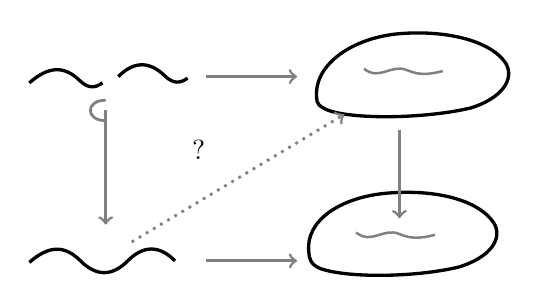
\begin{tikzpicture}[line width=1.2pt]
  \draw (-2.55,1.30) .. controls (-2.30,1.52) and (-2.10,1.52) .. (-1.90,1.32) .. controls (-1.80,1.23) and (-1.72,1.23) .. (-1.62,1.30);
  \draw (-1.42,1.38) .. controls (-1.22,1.58) and (-1.02,1.58) .. (-0.82,1.38) .. controls (-0.72,1.29) and (-0.64,1.29) .. (-0.54,1.36);
  \draw (-2.55,-0.98) .. controls (-2.30,-0.76) and (-2.10,-0.76) .. (-1.90,-0.96) .. controls (-1.70,-1.16) and (-1.50,-1.16) .. (-1.30,-0.96) .. controls (-1.10,-0.76) and (-0.90,-0.76) .. (-0.70,-0.96);
  \draw (1.10,1.10) .. controls (1.05,1.50) and (1.50,1.85) .. (2.10,1.92) .. controls (2.70,1.98) and (3.30,1.85) .. (3.50,1.55) .. controls (3.62,1.35) and (3.45,1.10) .. (3.05,0.98) .. controls (2.50,0.85) and (1.60,0.83) .. (1.25,0.95) .. controls (1.12,1.00) and (1.10,1.05) .. (1.10,1.10);
  \draw[gray,line width=0.9pt] (1.70,1.48) .. controls (1.90,1.32) and (2.05,1.55) .. (2.25,1.46) .. controls (2.40,1.40) and (2.50,1.40) .. (2.70,1.45);
  \draw (1.00,-0.85) .. controls (0.95,-0.45) and (1.40,-0.15) .. (2.00,-0.10) .. controls (2.60,-0.05) and (3.15,-0.18) .. (3.35,-0.48) .. controls (3.47,-0.68) and (3.30,-0.92) .. (2.90,-1.04) .. controls (2.35,-1.17) and (1.50,-1.18) .. (1.15,-1.06) .. controls (1.02,-1.01) and (1.00,-0.92) .. (1.00,-0.85);
  \draw[gray,line width=0.9pt] (1.60,-0.60) .. controls (1.80,-0.76) and (1.95,-0.53) .. (2.15,-0.62) .. controls (2.30,-0.68) and (2.40,-0.68) .. (2.60,-0.63);
  \draw[gray,line width=1pt,->] (-0.30,1.38) -- (0.85,1.38);
  \draw[gray,line width=1pt,->] (-0.30,-0.96) -- (0.85,-0.96);
  \draw[gray,line width=1pt,->] (-1.58,0.95) -- (-1.58,-0.50);
  \draw[gray,line width=1pt] (-1.58,1.08) .. controls (-1.84,1.08) and (-1.84,0.82) .. (-1.58,0.82);
  \draw[gray,line width=1pt,->] (2.15,0.70) -- (2.15,-0.42);
  \draw[gray,line width=1pt,->,dotted] (-1.25,-0.72) -- (1.45,0.90);
  \node at (-0.40,0.45) {$?$};
\end{tikzpicture}
\caption{\trSeparated{}性的\trValuativeCriteria。（依原书手绘图重绘。）}\label{fig:valuative-criterion-separatedness}
\end{figure}

\textbf{13.7.B.（练习）}\quad 设 $X$ 是一条整的诺特分离\trCurve。若 $p\in X$ 是一个正则的\trClosedPoint，则 $\OO_{X,p}$ 是一个\trDVR，于是每个正则点都在 $K(X)$ 上给出一个离散\trValuation。请用上一道练习证明：不同的点给出不同的离散赋值。

下面是这条\trValuativeCriteria{}背后的直觉（见\cref{fig:valuative-criterion-separatedness}）。我们把一个\trDVR{} $A$ 的 $\Spec$ 想成「一条\trCurve{}的\trGerm」，把 $\Spec K(A)$ 想成「挖去原点的\trGerm」（尽管它只是一个点！）。于是，这条\trValuativeCriteria{}说的是：若我们有一个从\trCurve{}的\trGerm{}到 $Y$ 的映射，并且有这个映射在挖去原点之处到 $X$ 的一个提升，那么把它从整个\trGerm{}提升起来的方式至多只有一种。当 $Y$ 是一个域的谱时，你可以把这理解为：单参数族的极限（若存在）必唯一。

例如，这抓住了 $k$ 上原点加倍了的\trAffineLine{}的映射毛病何在（\cref{fig:line-doubled-origin}）：我们取 $\Spec A$ 为\trAffineLine{}在原点处的\trGerm，考虑挖去原点的\trGerm{}到原点加倍了的\trAffineLine{}的映射。于是，这个映射延拓过原点的方式有两种选择。

\begin{figure}[htbp]
\centering
\begin{tikzpicture}[line width=1.2pt]
  \draw (-3.35,1.55) -- (-2.40,1.55);
  \draw (-2.15,1.55) -- (-1.20,1.55);
  \draw (0.60,1.55) -- (3.35,1.55);
  \draw[line width=1.1pt,fill=white] (2.10,1.55) circle (0.085);
  \draw (-3.35,-1.50) -- (-1.20,-1.50);
  \fill (2.10,-1.50) circle (0.075);
  \draw[gray,line width=1pt,->] (-0.60,1.55) -- (0.32,1.55);
  \draw[gray,line width=1pt,->] (-0.60,-1.50) -- (0.32,-1.50);
  \draw[gray,line width=1pt,->] (-2.15,1.30) -- (-2.15,-1.25);
  \draw[gray,line width=1pt,->] (2.10,1.30) -- (2.10,-1.25);
  \draw[gray,line width=1pt,->] (-1.88,-1.02) .. controls (-0.60,-0.15) and (0.50,0.70) .. (1.52,1.30);
  \draw[gray,line width=1pt,->] (-1.62,-1.26) .. controls (0.05,-0.60) and (1.10,0.15) .. (1.82,1.02);
  \node at (-1.15,0.38) {$\pi$};
  \node at (0.78,-0.55) {$\pi'$};
  \node at (0.02,0.10) {两种选择};
\end{tikzpicture}
\caption{原点加倍了的\trAffineLine{}不满足\trSeparated{}性的\trValuativeCriteria。（你也许会注意到\cref{fig:nonseparated-agreement}就嵌在这幅图里。）（依原书手绘图重绘。）}\label{fig:line-doubled-origin}
\end{figure}

\textbf{13.7.C.（练习）}\quad 请把这件事说精确：证明 $k$ 上原点加倍了的\trAffineLine{}到 $\Spec k$ 的映射不满足\trSeparated{}性的\trValuativeCriteria。（更早的论证见于\mbox{练习~11.2.I} 与\mbox{练习~11.3.C}。）

\textbf{13.7.2.}\ \extrahard\ \emph{行家注记：\trModuliSpace{}与\trSeparated{}性的\trValuativeCriteria。}\quad 若 $Y=\Spec k$，而 $X$ 是某类对象的（精细的）\trModuliSpace（这个术语我们在此不定义），那么 $X$（在 $\Spec k$ 上）的\trSeparatedness{}问题便有一个自然的解读：给定一个由「被刺穿的\trDVR」参数化的、由你的那些对象组成的\trFamily，把它延拓过闭点的方式是否总至多只有一种？

\textbf{13.7.3.}\ \emph{定理~13.7.1（\trSeparated{}性的\trValuativeCriteria{}的\trDVR{}版本）在簇情形下证明背后的想法。}\quad （一个方向已在\mbox{练习~13.7.A}中完成。）若 $\pi$ 不\trSeparated，我们的目标便是造出一幅形如 \eqref{eq:valuative-criterion-diagram}、且能以不止一种方式补全成 \eqref{eq:valuative-criterion-lift} 的图。若 $\pi$ 不\trSeparated，则 $\delta\colon X\to X\times_Y X$ 是一个并非闭嵌入的\trLocallyClosedEmbedding。

\textbf{13.7.D.（练习）}\quad 证明：你可以找到不在 $X\times_Y X$ 的对角线 $\Delta$ 中的点 $p$，以及 $\Delta$ 中的点 $q$，使得 $p\in\overline{q}$，而且不存在「介于 $p$ 与 $q$ 之间」的点（不存在异于 $p$ 与 $q$ 且满足 $p\in\overline{r}$ 与 $r\in\overline{q}$ 的点 $r$）。（\cref{ex:constructible-stable-specialization} 或许会带来一些启发。）

令 $Q$ 为给 $\overline{q}$ 赋以诱导的既约子概形结构所得的概形。令 $B=\OO_{Q,p}$ 为 $Q$ 在 $p$ 处的\trLocalRing。

\textbf{13.7.E.（练习）}\quad 证明：$B$ 是一个维数为 $1$ 的诺特局部整环。

若 $B$ 正则，那么我们就大功告成了：把包含态射 $Q\to X\times_Y X$ 与两个投射复合，诱导出同一个态射 $q\to X$（即 $\Spec\kappa(q)\to X$），但到 $B$ 上的延拓却彼此不同，其原因恰恰在于 $p$ 不在对角线之中。为了完成证明，需要证明 $B$ 的\trNormalization{}是诺特的；这正是我们需要「我们处理的是簇」这一假设之处，以便援引\mbox{练习~10.7.M}。然后在 $p$ 上方的任何一个素处取局部化（由 Lying Over 定理~8.2.5，这样的素是存在的），便得到所要的\trDVR{} $A$。

至于真正货真价实的证明，见 [Stacks, tag~0207] 或 [Gr-EGA, II.7.2.3]。

用更加强力的方式调用交换代数，我们便能在限制性假设弱得多的情形下证明一条\trValuativeCriteria。

\textbf{13.7.4.\ \trhTheorem{}（\trSeparated{}性的\trValuativeCriteria）。}\ ——\ \emph{设 $\pi\colon X\to Y$ 是一个拟分离\trMorphism。则 $\pi$ 是\trSeparated{}的，当且仅当：对任何\trValuationRing{} $A$，以及任何形如 \eqref{eq:valuative-criterion-diagram} 的图，使得 \eqref{eq:valuative-criterion-lift} 交换的\trMorphism{} $\Spec A\to X$ 至多只有一个。}

既然我已经没能把\trDVR{}版本证明完整，我也就提不起兴致去证明这个更难的事实了。其中一个方向——$\pi$ \trSeparated{}蕴涵判别法成立——其证明与\mbox{练习~13.7.A}中的论证完全一样。完整的证明见 [Stacks, tags~01KY 与 01KZ] 或 [Gr-EGA, II.7.2.3]。

\textbf{13.7.5.\ （泛闭性与）\trProperness{}的\trValuativeCriteria。}\quad \trProperness{}也有一条\trValuativeCriteria。它在哲学上有用，有时也直接有用，尽管我们并不需要它。它自然地来自\trSeparated{}性的\trValuativeCriteria{}与泛闭性的\trValuativeCriteria{}二者的结合。

\textbf{13.7.6.\ \trhTheorem{}（泛闭性与\trProperness{}的\trValuativeCriteria，\trDVR{}版本）。}\ ——\ \emph{设 $\pi\colon X\to Y$ 是局部诺特概形之间的一个有限型\trMorphism。则 $\pi$ 是\trUniversallyClosed{}的（相应地，固有的），当且仅当：对任何\trDVR{} $A$，以及任何图 \eqref{eq:valuative-criterion-diagram}，使得 \eqref{eq:valuative-criterion-lift} 交换的\trMorphism{} $\Spec A\to X$ 至少有一个（相应地，恰有一个）。}

证明见 [Gr-EGA, II.7.3.8]、[Ha1, Thm.~II.4.7] 或 [Gr-EGA$'$, I.5.5]。与定理~13.7.1 作一番比较，你就会相信这三条判别法自然地构成一个家族。

当 $Y$ 是一个域时，你可以把\trProperness{}的\trValuativeCriteria{}理解为：固有簇中单参数族的极限总是存在，而且唯一。这是对\trProperness{}这一观念的一个有用的直觉。

\textbf{13.7.F.（容易的练习）}\quad 请用\trProperness{}的\trValuativeCriteria{}证明：若 $A$ 是诺特环，则 $\mathbb{P}^n_A\to\Spec A$ 是固有的。（别被愚弄了：正因为这要用到\trValuativeCriteria，这是证明我们在定理~11.4.5 中已经证明过的事实的一条困难途径。）

\textbf{13.7.G.（练习；与\mbox{练习~13.7.B} 相对照）}\quad 设 $X$ 是一条不可约正则（诺特）\trCurve，在域 $k$ 上（相应地，在 $\mathbb{Z}$ 上）固有。请描述 $K(X)$ 上那些使 $k$（相应地，$\mathbb{Z}$）的元素赋值为 $0$ 的离散赋值与 $X$ 的闭点之间的一个双射。

\textbf{13.7.7.}\ \emph{行家注记。}\quad 有一个与\trSeparated{}性情形（注记~13.7.2）类似的模理论式解读：$X$ 是固有的，当且仅当把一个定义在\trDVR{}的刺穿谱上的\trFamily{}填补完整的方式总恰有一种。

\textbf{13.7.8.}\quad 最后，给出泛闭性与\trProperness{}的\trValuativeCriteria{}的一个更花哨的版本。

\textbf{13.7.9.\ \trhTheorem{}（泛闭性与\trProperness{}的\trValuativeCriteria）。}\ ——\ \emph{设 $\pi\colon X\to Y$ 是拟分离、有限型（因而拟紧）的\trMorphism。则 $\pi$ 是\trUniversallyClosed{}的（相应地，固有的），当且仅当下述条件成立。对任何\trValuationRing{} $A$ 与任何形如 \eqref{eq:valuative-criterion-diagram} 的图，使得 \eqref{eq:valuative-criterion-lift} 交换的\trMorphism{} $\Spec A\to X$ 至少有一个（相应地，恰有一个）。}

显然，\trProperness{}的\trValuativeCriteria{}是\trSeparated{}性的\trValuativeCriteria{}（定理~13.7.4）与泛闭性的\trValuativeCriteria{}二者的推论。证明见 [Stacks, tag~01KF] 或 [Gr-EGA, II.7.3.8]。

\textbf{13.7.10.\ 一般\trValuationRing{}的重要性。}\quad 尽管我们只深入讨论过\trDVR，但一般的\trValuationRing{}不应被视作事后补想的东西。\trSerre{}在一封信中向\trGrothendieck{}申明了这番道理\footnote{译注：来信按原书照录法语原文；紧随其后的一段中文，是笔者对作者英译的转译，个别字句从法文原信。}，[GrS, p.~125]：
\begin{quote}\itshape
Tu es bien sévère pour les Valuations!
Je persiste pourtant à les garder, pour plusieurs raisons:
d'abord une pratique: n rédacteurs ont sué dessus,
il n'y a rien à reprocher au fourbi,
on ne doit pas le vider
sans raisons très sérieuses (et tu n'en as pas).\,\ldots\
Même un noethérien impénitent a besoin
des valuations discrètes, et de leurs extensions;
en fait, Tate, Dwork, et tous les gens p-adiques
te diront qu'on ne peut se limiter au cas discret
et que le cas de rang 1 est indispensable;
à ce moment, les méthodes noethériennes
deviennent un vrai carcan,
et on comprend beaucoup mieux
en rédigeant le cas général
que uniquement le cas de rang 1.\,\ldots\
Il n'y a pas lieu d'en faire un plat,
bien sûr,
et c'est pourquoi j'avais vivement
combattu le plan Weil initial
qui en faisait le théorème central
de l'Algèbre Commutative,
mais d'autre part il faut le garder.\footnote{原书法语原文中「j'avias」「gen」「leurs extension」「devient」四处显系排印笔误（当为「j'avais」「gens」「leurs extensions」「deviennent」），径改。——译者注}
\end{quote}
\begin{quote}\itshape
你对赋值太苛刻了！然而我坚持要把它们保留下来，理由有好几条，其中第一条是实际操作层面的：$n$ 位编辑已经为它们流过汗了，这件成品没有什么可指摘之处，没有非常严肃的理由就不该把它清空（而你并没有这样的理由）。\ldots\ 就连一个死不悔改的诺特派也需要离散赋值及其扩张；事实上，\trTate、\trDwork，以及所有\trPadic{}人士都会告诉你：人不能把自己局限在离散情形，而秩 $1$ 的情形是不可或缺的；到了那种时候，诺特式方法就成了一副真正的枷锁，而通过撰写一般情形（而不只是秩 $1$ 情形），你能理解得好得多。\ldots\ 当然，犯不着为此小题大做，也正因如此，我当年曾激烈地反对\trWeil{}最初那个把它立为交换代数中心定理的计划；但另一方面，它必须保留。
\end{quote}


\section{\hard\ \trRegular\trLocalRing{}的进阶事实}

正则局部环几乎具备你想要的每一种好性质，但其中一些需要下苦功。我们现在来讨论几条更为精致的事实，它们或许能帮你夜里睡得安稳。

\textbf{13.8.1.\ 正则局部环的诸\trLocalization{}都是\trRegular\trLocalRing。}

\textbf{13.8.2.\ 事实（[E, Cor.~19.14]、[Mat2, Thm.~19.3]）。}\ ——\ \emph{若 $(A,\mathfrak{m})$ 是一个\trRegular\trLocalRing，则 $A$ 在任一\trPrimeIdeal{}处的\trLocalization{}也是\trRegular\trLocalRing。}

（我们并不需要这条结果，因此也不会去证明它。）这条重大定理在\trCommutative{}代数中曾是一个长期悬而未决的问题，直到 \trSerre{}与 Auslander--Buchsbaum 用同调方法将其解决。

于是，要检验 $\Spec A$ 是否正则（$A$ \trNoetherian），只需在诸\trClosedPoint{}（即诸\trMaximalIdeal{}）处检验就够了。假定事实~13.8.2（并使用\mbox{练习~5.1.E}），你便可以通过在闭点处检验来检验一个\trNoetherian{}概形的正则性。

我们将证明事实~13.8.2 的两个重要特例。第一个你现在就能动手做。

\textbf{13.8.A.（练习）}\quad 设 $X$ 是一个\trNoetherian{}、维数为 $1$ 的概形，并且在其诸\trClosedPoint{}处正则。证明：$X$ 是\trReduced{}的。进而（在不援引事实~13.8.2 的前提下）证明：$X$ 是正则的。

第二个重要特例将在 \S21.6.2 中得到证明：

\textbf{13.8.3.\ \trhTheorem{}。}\ ——\ \emph{若 $X$ 是完全域 $k$ 上的一个\trFiniteType{}概形，并且在其诸\trClosedPoint{}处正则，则 $X$ 正则。}

更一般地，\mbox{练习~21.6.B}将证明：若 $A$ 是完全域上一个有限型代数的\trLocalization，则事实~13.8.2 成立。

\textbf{13.8.B.（练习：推广\mbox{练习~13.3.E}）}\quad 设 $k$ 是特征为 $0$ 的\trAlgClosedField。假定定理~13.8.3，证明：$\mathbb{P}^n$ 中存在每个正次数 $d$ 的正则\trHypersurface。（与\mbox{练习~13.3.E}一样，尽管随意放宽假设。）

\textbf{13.8.4.\ 正则局部环都是\trUFD、整闭的，并且是 \trCM{}的。}

\textbf{13.8.5.\ 事实（Auslander--Buchsbaum 定理）。}\ ——\ \emph{正则局部环都是\trUFD。}

（这是一条艰难的定理，所以我们不证明它，因而也不会去使用它。证明可参看 [E, Thm.~19.19]、[Mat2, Thm.~20.3] 或 [Gr-EGA, IV$_4$.21.11.1]；至于\trVariety{}这一特殊情形，则见 [Mu7, \S III.7]。）从而正则概形都是\trFactorial{}的，故由\mbox{练习~5.4.F}是\trNormal{}的。

\textbf{13.8.6.}\ \emph{\trhRemark{}：\trFactoriality{}弱于\trRegularity。}\quad 「正则蕴涵唯一分解」这条蕴含关系是严格的。下面就是一个表明此事的例子。设 $k$ 是特征不为 $2$ 的\trAlgClosedField。令 $A=k[x_1,\dots,x_n]/(x_1^2+\cdots+x_n^2)$（对照\mbox{练习~5.4.I}）。注意 $\Spec A$ 显然在原点处\trSingular。在\mbox{练习~15.5.R}中，我们将证明当 $n\ge5$ 时 $A$ 是一个\trUFD，故 $\Spec A$ 是\trFactorial{}的。特别地，$A_{(x_1,\dots,x_n)}$ 是一个\trNoetherian\trLocalRing，它是\trUFD，却不是正则的。（更一般地，\trGrothendieck{}对 P.~Samuel 一个猜想的证明蕴涵：一个\trNoetherian\trLocalRing，倘若它是一个\trCompleteIntersection（特别地，是一个\trHypersurface），并且在余维数至多 $3$ 处\trFactorial，则它必是\trFactorial{}的，[SGA2, Exp.~XI, Cor.~3.14]。一份更简短且多少更初等的证明见 [CL]。）

\textbf{13.8.7.}\ \emph{正则局部环是整闭的。}\quad Auslander--Buchsbaum 定理（事实~13.8.5）蕴涵：正则局部环是整闭的（由\mbox{练习~5.4.F}）。我们将在 \S26.3.5 中证明这件事（不诉诸事实~13.8.5）。

\textbf{13.8.8.}\ \emph{正则局部环是 \trCM{}的。}\quad 在 \S26.2.5 中，我们将证明正则局部环都是 \trCM{}的（这个概念将在第 26 章中定义）。


\section{\hard\ 滤过环与模、\trArtin--\trRees{}引理}

我们以讨论\trArtin--\trRees{}引理~13.9.3 来为第 13 章收尾，这条引理曾被用来证明命题~13.5.2。\trArtin--\trRees{}引理推广了命题~13.5.2 背后的直观：在一点处解析地为零的任何函数，实际上都在该点的一个开\trNeighborhood{}内消失（\S13.5.3）。由于我们日后会用到它，也由于能在其他情境中认出它来是件有用的事，我们将对它作颇为细致的讨论。

\textbf{13.9.1.}\ \emph{\trhDefinition{}。}\quad 设 $I$ 是环 $A$ 的一个\trIdeal。$A$-模 $M$ 的一个递降滤过
\begin{equation*}\tag{13.9.1.1}\label{eq:i-filtration}
M=M_0\supset M_1\supset M_2\supset\cdots
\end{equation*}
称为\textbf{一个 $I$-\trFiltration}（$I$-filtration），若对一切 $d$、$n\ge0$ 都有 $I^dM_n\subset M_{n+d}$。一个例子是\textbf{$I$-进滤过}（$I$-adic filtration），即 $M_k=I^kM$ 的情形。我们称一个 $I$-\trFiltration{}是\textbf{$I$-稳定}的（$I$-stable），若存在某个 $s$，使得对一切 $d\ge0$ 都有 $I^dM_s=M_{d+s}$。例如，$I$-进滤过就是 $I$-稳定的。

令 $A(I)_\bullet$ 为\trGradedRing{} $\bigoplus_{n\ge0}I^n$（约定 $I^0=A$）。它称为 $A$ 中\trIdeal{} $I$ 的\textbf{\trRees{}代数}（Rees algebra），尽管我们并不需要这个术语。定义 $M(I)_\bullet:=\bigoplus_n M_n$。它自然是 $A(I)_\bullet$ 上的一个\emph{\trGradedModule}。

\textbf{13.9.2.\ \trhProposition{}。}\ ——\ \emph{设 $A$ \trNoetherian，$M$ 是有限生成的 $A$-模，而滤过~\eqref{eq:i-filtration} 是一个 $I$-\trFiltration。则 $M(I)_\bullet$ 是有限生成的 $A(I)_\bullet$-模，当且仅当滤过~\eqref{eq:i-filtration} 是 $I$-稳定的。}

\emph{证明。}\ 注意 $A(I)_\bullet$ 是\trNoetherian{}的（由\mbox{练习~4.5.G(b)}，因为 $A$ 是\trNoetherian{}的，而 $I$ 是有限生成的 $A$-模）。

先设 $M(I)_\bullet$ 在\trNoetherian{}环 $A(I)_\bullet$ 上有限生成，从而它是\trNoetherian{}的。考虑由 $A(I)_\bullet$-\trSubmodule{}构成的递增链，其第 $k$ 项 $L_k$ 为
\[
M\oplus M_1\oplus M_2\oplus\cdots\oplus M_k\oplus IM_k\oplus I^2M_k\oplus\cdots
\]
（它在到达 $M_k$ 之前与 $M(I)_\bullet$ 一致，随后便「$I$-稳定化」）。由\trNoetherian{}性，这条链必将稳定。但 $\bigcup L_k=M(I)_\bullet$，于是对某个 $s\in\mathbb{Z}^{\ge0}$ 有 $L_s=M(I)_\bullet$，从而对一切 $d\ge0$ 都有 $I^dM_s=M_{s+d}$——\eqref{eq:i-filtration} 是 $I$-稳定的。

另一个方向：设对某个固定的 $s$ 与一切 $d\ge0$ 都有 $M_{d+s}=I^dM_s$。那么 $M(I)_\bullet$ 在 $A(I)_\bullet$ 上由 $M\oplus M_1\oplus\cdots\oplus M_s$ 生成。但每个 $M_j$ 都有限生成，故 $M(I)_\bullet$ 的确是一个有限生成的 $A(I)_\bullet$-模。\hfill$\square$

\textbf{13.9.3.\ \trArtin--\trRees{}引理。}\ ——\ \emph{设 $A$ 是\trNoetherian{}环，而 \eqref{eq:i-filtration} 是有限生成 $A$-模 $M$ 的一个 $I$-稳定滤过。设 $L\subset M$ 是一个\trSubmodule，并令 $L_n:=L\cap M_n$。则}
\[
L=L_0\supset L_1\supset L_2\supset\cdots
\]
\emph{是 $L$ 的一个 $I$-稳定滤过。}

\emph{证明。}\ 注意 $L_\bullet$ 是一个 $I$-\trFiltration，因为 $IL_n\subset IL\cap IM_n\subset L\cap M_{n+1}=L_{n+1}$。此外，$L(I)_\bullet$ 是有限生成的 $A(I)_\bullet$-模 $M(I)_\bullet$ 的一个 $A(I)_\bullet$-\trSubmodule，从而由\mbox{练习~3.6.Y}它是有限生成的（因为 $A(I)_\bullet$ 是\trNoetherian{}的，见命题~13.9.2 的证明）。\hfill$\square$

一个重要的特殊情形如下。

\textbf{13.9.4.\ \trhCorollary{}。}\ ——\ \emph{设 $I\subset A$ 是\trNoetherian{}环的一个\trIdeal，$M$ 是有限生成的 $A$-模，而 $L$ 是一个\trSubmodule。则对某个整数 $s$，对一切 $d\ge0$ 都有 $I^d(L\cap I^sM)=L\cap I^{d+s}M$。}

\trhWarning{}：对于一切 $d$ 而言，$I^dL=L\cap I^dM$ 未必成立。（你能想出这个陈述的一个反例吗？）

\emph{证明。}\ 对滤过 $M_n=I^nM$ 应用\trArtin--\trRees{}引理~13.9.3。\hfill$\square$

\textbf{13.9.A.（练习：\trKrull{}交定理）}\quad
\begin{enumerate}[label=(\alph*)]
\item 设 $I$ 是\trNoetherian{}环 $A$ 的一个\trIdeal，而 $M$ 是有限生成的 $A$-模。证明：存在某个满足 $a\equiv1\pmod{I}$ 的 $a$，使得 $a\bigcap_{j=1}^{\infty}I^jM=0$。（提示：取 $L=\bigcap_{j=1}^{\infty}I^jM$、$M_n=I^nM$，应用\trArtin--\trRees{}引理~13.9.3。证明 $L=IL$，然后应用\trNakayama{}引理的第一种版本（引理~8.2.8）。）
\item 证明：若 $A$ 是\trNoetherian\trIntegralDomain{}或\trNoetherian\trLocalRing，而 $I$ 是一个\trProperIdeal，则 $\bigcap_{j=1}^{\infty}I^j=0$。特别地，你将由此证得命题~13.5.2：若 $(A,\mathfrak{m})$ 是\trNoetherian\trLocalRing，则 $\bigcap_i\mathfrak{m}^i=0$。
\end{enumerate}

\textbf{13.9.B.（练习）}\quad 请把下面这件事精确化，并证明之（从而印证 \S13.5.3 的直观）：若 $X$ 是一个\trLocally\trNoetherian{}概形，而 $f$ 是 $X$ 上在一个点 $p\in X$ 处解析地为零的函数，则 $f$ 在 $p$ 的一个（扎里斯基）开\trNeighborhood{}内消失。

